% \documentclass[a4paper, 10pt]{IEEEtran}
\documentclass[10pt]{article}

% packages
  \PassOptionsToPackage{hyphens}{url}\usepackage[colorlinks,linkcolor=blue,citecolor=blue,urlcolor=blue]{hyperref}
  \usepackage[all]{hypcap}

  % \usepackage[colorinlistoftodos]{todonotes}
  \usepackage[english]{babel}
  % \usepackage[margin=1in]{geometry}
  \usepackage[utf8]{inputenc}

  \usepackage{titling}

  \usepackage{amsmath}
  \usepackage{amssymb}
  \usepackage{upgreek}

  \usepackage{booktabs}
  \usepackage{tablefootnote}
  \usepackage{multirow}
  \usepackage{color}
  
  \usepackage{enumitem}
  \usepackage{float}
  \usepackage{listings}

  \usepackage{palatino}
  \usepackage[T1]{fontenc}

  \usepackage{calc}

  \usepackage{siunitx}

  % \usepackage{subfig}

  \usepackage{colortbl}
  \usepackage{pdfpages}
  \usepackage{textcomp}
  \usepackage{xspace}
  \usepackage{csquotes}
  \usepackage{siunitx}
  \usepackage{appendix}

  \usepackage{graphicx}
  \usepackage{subfigure}

  \usepackage{adjustbox}
  \usepackage{changepage}
  \usepackage[pass]{geometry}

  \usepackage{blindtext}
  % \usepackage{titlesec}
  % \usepackage[xindy]{glossaries}
  % \usepackage[normalem]{ulem}

  \usepackage{import}
  \graphicspath{{pics/}{../pics/}}


  % \setlist{noitemsep}

  \setcounter{secnumdepth}{5}
  \setcounter{tocdepth}{5}

  \usepackage[numbers]{natbib}
  \bibliographystyle{plainnat}

% defines
  \definecolor{mygray}{rgb}{0.9,0.9,0.9}
  \lstset{
      basicstyle=\ttfamily\footnotesize,
      tabsize=2,
      % backgroundcolor=\color{mygray},
      % numbers=left
  }

  % %% disable figures
  % \usepackage{comment}
  % \excludecomment{figure}
  % \let\endfigure\relax
  % %% disable figuress
  % \newcommand{\done}{\checkmark?}
  \newcommand{\done}{}
  % \newcommand{\readonemoretime}{\textsc{r}!}
  \newcommand{\readonemoretime}{}

  % \newcommand{\TI}{ASILD1 (TI TMS570)\xspace}
  \newcommand{\TI}{TMS570\xspace}
  % \newcommand{\ST}{ASILD2 (ST SPC570)\xspace}
  \newcommand{\ST}{SPC570\xspace}
  \newcommand{\NXP}{QM target\xspace}

  \newcommand{\unroll}{\texttt{unroll}\xspace}
  \newcommand{\auth}{\texttt{auth}\xspace}
  \newcommand{\authone}{\texttt{auth-1}\xspace}
  \newcommand{\authtwo}{\texttt{auth-2}\xspace}
  \newcommand{\jtag}{JTAG\xspace}

  \newcommand{\UU}{\textsc{uu}\xspace}
  \newcommand{\UD}{\textsc{ud}\xspace}
  \newcommand{\SU}{\textsc{su}\xspace}
  \newcommand{\SD}{\textsc{sd}\xspace}
  \newcommand{\R}{\textsc{r}\xspace}

  \newcommand{\Q}{\textsc{q}\xspace}
  \newcommand{\Qa}{\textsc{q}a\xspace}
  \newcommand{\Qb}{\textsc{q}b\xspace}

  \newcommand{\errorpin}{\textsc{eout}\xspace}
  \newcommand{\errorpinzero}{\textsc{eout0}\xspace}
  \newcommand{\errorpinone}{\textsc{eout1}\xspace}

  % \newcommand{\note}[2]{[#1] \todo{#2} }

  % autoref fixes
  \newcommand*{\Appendixautorefname}{Appendix}
  \newcommand{\subfigureautorefname}{\figureautorefname}

  \renewcommand*{\sectionautorefname}{Section}
  % \renewcommand*{\thesection}{\Roman{section}}
  % \renewcommand*{\thesubsection}{\thesection.\Alph{subsection}}

  \let\subsectionautorefname\sectionautorefname
  \let\subsubsectionautorefname\sectionautorefname


  % hypenation
  \hyphenation{lock-step}

  %keyword command
  \providecommand{\keywords}[1]{\textbf{\textit{Keywords---}}#1}

% titlepage
  \title{SAFETY $\neq$ SECURITY \\ A SECURITY EVALUATION OF STATE OF THE ART AUTOMOTIVE MICROCONTROLLERS}
  \author{}
  \date{}

\begin{document}
  \pagenumbering{gobble}

\begin{titlepage}
  \begin{center}

  \vspace*{-2cm}

  
\includegraphics[width=3cm]{rulogo_notext.pdf}\\
  \vspace*{0.2cm}
  {\scshape\LARGE Radboud University\par}\vspace{1.5cm} % University name

  \textsc{\Large Master's Thesis \\ Computing Science}\\[1.5cm] % Thesis type

  % \HRule \\[0.4cm] % Horizontal line
  % \hline
  \vspace{0.4cm}\noindent\rule{\textwidth}{0.4pt} \vspace{0.6cm}\\
  {\huge \bfseries SAFETY $\neq$ SECURITY}\\{\LARGE A security evaluation of state of the art automotive microcontrollers \\} 
  \vspace{0.6cm} \noindent\rule{\textwidth}{0.4pt}\vspace{1cm} \\
  % \HRule \\[1.5cm] % Horizontal line
   
  \begin{minipage}[t]{0.4\textwidth}
  \begin{flushleft} \large
  \emph{Author:}\\
  Nils Wiersma \\
  \end{flushleft}
  \end{minipage}
  \begin{minipage}[t]{0.5\textwidth}
  \begin{flushright} \large
  \emph{Supervisors:} \\
  dr. Lejla Batina \\
  dr. Ilya Kizhvatov \\ \ \\
  \emph{External supervisors:} \\
  Ramiro Pareja Veredas  \\
  Albert Spruyt \\
  \end{flushright}
  \end{minipage}\\
   
  \vfill

  % \large \textit{A thesis submitted in fulfillment of the requirements\\ for the degree of \degreename}\\[0.3cm] % University requirement text
  % \textit{in the}\\[0.4cm]
  % \groupname\\\deptname\\[2cm] % Research group name and department name
   
  %\vfill

  {\large May 2, 2017}\\[4cm] % Date
  %\includegraphics{Logo} % University/department logo - uncomment to place it
   
  \vfill
  \end{center}
\end{titlepage}

\begin{titlingpage}
  % \maketitle

  \section*{Abstract}
  % \begin{abstract}
    \noindent Electronic systems are increasingly replacing both `dumb' automotive functionalities -- such as opening a window and locking your car -- as well as replacing driver actions by introducing more and more `smart' functionalities -- such as cruise control, automatic parking and complete autopilot systems. Many of these functionalities, especially those related ensuring the safety of passengers, require high levels of fault tolerance in the electronic systems. 
    The ISO26262 standard on functional safety in road vehicles, introduced in 2011, proposes the ASIL (Automotive Safety Integrity Level) scheme, a risk classification system for functional safety. ASIL-D certified systems -- the highest level of assurance -- are required to have several safety mechanisms in place to achieve fault tolerance. One of these mechanisms is implementing a second redundant CPU inside the microcontroller, operating in a lockstep configuration with the primary CPU. Other mechanisms found in this standard include protections on the memory level, such as parity checks, ECC and memory duplications. Although the ASIL-D requirements do not mention anything about security, it is commonly thought that the lockstep configuration should detect low-level hardware attacks like fault injection in the fault injection literature. \\
    
    \noindent In this work, we analyze two recent examples of ASIL-D certified microcontroller from different vendors that implement, among others, the lockstep mechanism. We find that of these mechanisms, lockstep is the most effective mechanism against some the typical targets of a fault injection attack. However, we also find that these mechanisms do not adequately protect against fault injection attacks. Moreover, we are able to apply fault injection attacks to unlock the JTAG protection of an ASIL-D chip, with the help of power analysis. 
    
  % \end{abstract}
  \vspace{2.5cm}
  % \vfill  
  \noindent {\normalsize \keywords{fault injection, fault tolerance, hardware redundancy, ISO26262, ASIL-D, microcontroller unit, safety mechanisms,  countermeasures, lockstep, safety, security, automotive}}

\newpage

  \tableofcontents
\end{titlingpage}



\pagenumbering{arabic}

\newpage
\section{Introduction }

    Recent statistics estimate that modern automobiles contain anywhere between 50 to 70 \cite{koscher_experimental_2010}, or up to 100 \cite{brians_cyber_2016} different Electronic Control Units\footnote{sometimes referred to as Electronic Computing Unit or Engine Control Unit} (ECU). 
    They are used to implement functionalities as simple as opening a window on a button press, or to implement functionalities as complicated as Vehicle to Vehicle communications and autonomous driving systems. They can offer non-critical functionalities such as controlling the windscreen wipers, or highly critical functionalities like making sure airbags are deployed in case of emergency. 
    At the heart of these ECUs one often finds microcontroller units. % to control the ECU that provides these different kinds of functionalities. 
    Given the criticality of the functionalities they provide, stringent requirements in terms of safety are placed upon them. 
    The \citet{iso26262} standard on functional safety for road vehicles also recognizes the pivotal part that microcontroller units play in the ecosystem of an automobile, evidenced by the special attention they receive in \citet[Annex A]{iso26262-10} and \citet[Annex D]{iso26262-5}. The first explains how the standard can be applied on the microcontroller level, even when it is not yet part of an actual component, but when it is considered a Safety Element out of Context. The latter gives a number of examples of safety mechanisms\footnote{technical solutions that detect or control faults, to maintain a safe state \cite{iso26262-1}} that could be implemented to combat different fault sources.

    Some of the safety mechanisms that are proposed in \citet[Annex D]{iso26262-5} are also found in the security literature  \cite{bar-el_sorcerers_2006} that relates to fault injection attacks as potential countermeasures against these attacks. Having these mechanisms available in products meant for mass production offers an interesting opportunity to evaluate the effect they have on %fault injection 
    security. Additionally, claims of safety could be extended to claims of security based on this parallel in measures between both contexts -- for example, \citet{burton_automotive_2012} propose to extend the \citet{iso26262} standard with security goals to achieve this. Such an evaluation is presented in this work.% indicates the risks and pitfalls of doing so.

    


  \newpage
  \subsection{Research questions }
  \label{sec:questions}

    The investigation of the effectiveness of the safety mechanisms as countermeasures against fault injection attacks found inside these high assurance microcontrollers is formulated into the following research question: 

    \begin{itemize}
      \item[\Q :] What is the current state of the security of the microcontrollers used in the automotive industry with respect to fault injection attacks?
    \end{itemize}

    \noindent This question will be answered in two parts. The first part illustrates what exactly security means in the automotive context, by providing an answer to the following question, along with its subquestions:

    \begin{itemize}
      \item[\Qa :] What are the common automotive attacker scenarios that can utilize fault injection attacks?
      \begin{itemize}
        \item Who are the actors?
        \item Which assets do they target?
        \item How does microcontroller security fit in this scenario?
      \end{itemize}
    \end{itemize}

    \noindent In order to answer the second part of the research question, an answer will be provided to the following question:

    \begin{itemize}
      \item[\Qb :] To what extent are advanced hardware attacks that use fault injection mitigated by safety mechanisms found in the automotive industry?
    \end{itemize}

    \noindent The purpose of \Qa is to establish a security context in which the the results of \Qb can be placed. Both together provide an answer to \Q. 

  \newpage
  \subsection{Contribution}

    Contemporary automotive security research is primarily interested in remotely exploitable attacks \cite{checkoway_comprehensive_2011}. And for good reason: the many wireless interfaces present in a modern automobile -- WiFi, Bluetooth, cellular, Tire Pressure Monitoring Systems -- present a serious attack surface \cite{brians_cyber_2016,smith_car_2016}. This surface will only increase to grow as new connectivity functionalities are added, such as Vehicle to Vehicle networks. Not to mention that the internal network protocols used by the many components are typically inherently insecure. 
    As the industry will move to harden the security at these fronts, attackers will shift to alternative methods of compromising these components. One such method is through fault injection as presented in this work. 

    Some work \cite{kanekawa_fault_1998,tummeltshammer_power_2009} on the effect of fault injection on the same countermeasures that are found in modern automotive microcontroller units has been done -- in particular through power glitching. They find that the countermeasures under their consideration (lockstep and error correction and detection codes) are highly successful as countermeasures in their experiments and in fact detect all of the faults they induce with power glitching. Contrary to their findings, this work presents findings showing that undetected faults are possible with the presence of such countermeasures and alerts on the risks of relying solely on these countermeasures as a defense against fault injection attacks.

    These findings are obtained through a security evaluation that involves two types of settings. 
    First, a series of characterization experiments are performed on two state of the art automotive microcontroller targets, who aim to ascertain the highest level of safety assurance as defined by the \citet{iso26262} standard. This indicates the general resilience of such targets against fault injection attacks. Secondly, a realistic attack is presented on one of the targets that attempts to (and succeeds in) bypass(ing) the mechanism that protects access to the debugging interface. This shows that with the presence of advanced hardware countermeasures fault injection is still a feasible attack method. 

  


  \newpage
  \subsection{Outline }

    This thesis is structured as follows:

    \begin{description}
      \item[\autoref{sec:background}] provides the reader with all the background in the areas of safety, security, ISO26262 and fault injection. This includes a discussion of the differences between safety and security, a summary of different techniques for performing fault injection and an overview of the common mechanisms encountered in microcontrollers specific for the automotive context.
      \item[\autoref{sec:attacker-scenarios}] describes several attacker scenarios applicable in the automotive context, relevant to the attacks outlined in this work, to illustrate the impact of fault injection attacks. 
      \item[\autoref{sec:methodology}] details all the different tools that have been used for this work and summarizes the important details of the targets under consideration. It also explains the setups in which these two come together. Furthermore, it will outline the steps of the experiments that have been performed.
      \item[\autoref{sec:characterization-results}] presents and discusses the results of the characterization experiments. It discusses the effectiveness of the mechanisms implemented by the targets as countermeasures against fault injection attacks, as well as the effect that different parameters have on the success rate of fault injections.
      \item[\autoref{sec:realistic-attack}] presents the same as \autoref{sec:characterization-results}, but for the realistic attack concerning debugging interface protection. It also goes into detail on some of the preparatory steps of this attack, in particular the part that requires power analysis.
      \item[\autoref{sec:mitigations+futurwork}] provides some recommendations on how levels of mitigation can be increased and provides some pointers on future work.
      \item[\autoref{sec:conclusion}] summarizes all the primary findings of this work.
    \end{description}
    \vfill
    \begin{description}
      \item[\autoref{apdx:results}] contains a comprehensive table of the results of the various experiments performed.
      \item[\autoref{apdx:parameters}] contains a comprehensive table of the parameter settings used to obtain these results.
      \item[\autoref{apdx:st-power}] contains a the separate results of the unsuccessful attack on the \ST.
    \end{description}

\newpage
\section{Background and related work }
\label{sec:background}

  This section presents the background and related work for this work. It addresses the topics of security, safety, fault injection and countermeasures.

  \subsection{Safety and security }

    In this work the effect of safety mechanisms that are designed with the purpose of safeguarding reliability and safety are considered as potential countermeasures to ensure security. Safety and security are terms that are easily conflated. This section will address differences and similarities between safety and security and any other term of importance, in order to avoid any confusion and clearly define the scope of this work.

    Safety is typically associated with hazards, while security deals with threats. Hazards are the cause of physical injury. When thinking about safety, health and physical well-being of a person are the central concern. For \citet{iso26262-1}, this harm has to be specifically caused by the malfunctioning behavior of an electric or electronic system. The threats that security deals with, on the other hand, is a much broader term. It captures physical harm, but also includes other consequences such as loss of (intellectual) property, financial loss or intrusion of privacy. Safety and security might overlap in some cases, complement each other in others and they can even contradict each other \cite{burton_automotive_2012}, so careful consideration is appropriate. ISO26262 further specifies \emph{functional} safety, which is a quantification of safety, defined to be the \enquote{absence of unreasonable risk due to hazards caused by an electric or electronic system.} \cite{iso26262-1}

    A central cause of malfunctioning behavior of a system in both safety and security context is a fault. A distinction is typically made between transient faults -- faults that are cleared upon a reset -- and destructive faults -- permanent changes to a target. \cite{bar-el_sorcerers_2006} 
    In \citet{iso26262-1} more distinctions between different kinds of faults are made, illustrated by a flow diagram found in ISO26262-5 \cite{iso26262-5}. The first distinction made is based on the nature of their cause:

    \begin{description}
      \item[Systematic failures] are the result of a condition that is completely deterministic. The only way to fix these failures is by patching the cause.
      \item[Random hardware failures] are the unpredictable events that happen during the lifetime of the device. 
    \end{description}

    \noindent A second distinction is made based on the amount of faults it takes to violate a safety goal\footnote{safety goals are the top-level safety requirements that are established after performing hazard analysis and risk assessment \cite{iso26262-1}}:

    \begin{description}
    \item[Single-point faults] only require a single fault to violate a safety goal.

    \item[Multiple-point faults] require more than a single fault to occur. Note that any fault that needs more than two faults to violate a safety goal are automatically classified as a safe fault, unless they are shown to be relevant.
    \end{description}


    \noindent Depending on how a safety mechanism positions itself relative to a safety goal and a fault, another distinction is made: 

    \begin{description}
    \item[Safe faults]  are faults that might or might not be covered by a safety mechanism, but the effect does not violate any safety goal.

    \item[Single-point faults] violate a safety goal, and no safety mechanisms are in place to cover this fault.

    \item[Residual faults] violate a safety goal, while a safety mechanisms is in place to cover this fault, but this mechanism does not prevent the violation of the safety goal.
    \end{description}

    \noindent Finally, separate categories exist for \textbf{detected} (by the mechanism), \textbf{perceived} (by the driver) and \textbf{latent} (not detected nor perceived) faults. Note that only multiple-point faults can be considered latent. 

    In order to classify the faults that are measured in the experiments of this work, a categorization of faults has been made that has some overlap with the ISO26262 categorization mentioned here. This is discussed in \autoref{sec:attackstrategy} and the overlap is outlined in \autoref{tab:categories}.

    Safety mechanisms are considered a subset of safety measures. Their specific goal is to avoid or control aforementioned in the case of systematic failures, while random hardware failures merely have to be detected or controlled, or their harmful effect must be mitigated. This definition is slightly more specific than the more broad countermeasure, typically defined as solution to avoid, detect and/or  correct faults \cite{bar-el_sorcerers_2006}.

    ISO26262-9 \cite{iso26262-9} defines different Automotive Safety Integrity Integrity Levels (ASILs). These levels are assigned to safety goals. %, depending on certain parameters. 
    The different levels are classified using A through D, with D being the most stringent. For a system to achieve compliance with a certain level, it must cover all the safety goals specified throughout ISO26262 \cite{iso26262} associated with that level. 
    The lowest of compliance level is Quality Management, or QM, requiring only basic quality management. For an overview of this system, see \autoref{tab:ASIL}.

    \begin{table}[H]
        \centering
        \begin{tabular}{rccccccc}
        \toprule
        Assurance level &&& Low &  \multicolumn{3}{c}{$\xrightarrow{\hspace*{3cm}}$}      & High \\
                        % &&& &&&&\\
        Category        &&& QM  & ASIL-A & ASIL-B & ASIL-C & ASIL-D \\
        % \cmidrule{1-6}
        \bottomrule
        \end{tabular}
        \caption{ASIL categories} 
        \label{tab:ASIL}
    \end{table}

    \noindent These levels have been used to select the targets discussed in \autoref{sec:targets}.%\todo{tabular overview?}

  \subsection{Fault injection and security }
  \label{sec:fi+security}

    Fault injection \emph{testing} is explicitly mentioned in \citet{iso26262-5} as a test to verify completeness and correctness of a safety mechanism. In the context of safety, the faults that are being tested against are the result of the hostile environment in which the system resides. They are unintentional and abnormal conditions, which can be systematic or be of a random nature. When faults are injected as an attack, they are no longer unintentional. They are caused by \textbf{glitches} that are deliberately placed, precisely timed and carefully tuned.
    Depending on the resolution of the tools that inject the glitch and parameters of the target such as speed and size, the \textbf{faults} that these glitches achieve can even be considered completely systematic, rather than random. 

    The immediate effect a glitch has on a microcontroller is very hard to determine. For an attacker this is typically not a problem, as he is interested in the effect of the glitch on the instructions that it executes -- the fault. For a manufacturer, the immediate effect is of greater interest, as it aids in mitigating the effect of glitches.  When only the fault that a glitch causes is of interest -- as is the case for this work -- one can construct series of characterization experiments to determine the effect this fault has on instructions and values that are being loaded into a core. These experiments are done on small code snippets in a controlled environment, to reduce the number of variables that can have an influence on the observable result of a glitch. 
    An overview of a set of such experiments in the context of power glitching is given in \citet{spruyt_building_2012}. \citet{balasch_-depth_2011} details the effects of clock glitching on an 8-bit smartcard microcontroller. For the effects of EM glitching, \citet{moro_electromagnetic_2013} discusses the results of EM glitching on a 32-bit microcontroller. In \citet{aarts_electromagnetic_2013}, several smartcards have been characterized using EM glitching, and these results are compared against results of optical glitching.

    In general, the purpose of a fault injection attack is to cause non-destructive, transient faults, also known as Single Event Upsets or a `bit-flip'. They allow for repeatable experiments, leave the target functional after the attack and provide all the tools required for the goals outlined in \autoref{sec:attacker-scenarios}. Multiple bit-flips can be combined, forming a Multiple Event Upset. Other more destructive and permanent faults are not considered in this work. \cite{bar-el_sorcerers_2006}

    Bit-flips are the basic faults on which a fault injection attack is built. These flips occur in values that can be interpreted as instructions, addresses, or as a numeric value. Altering one value might indirectly affect the rest of that execution -- for example, a fault in an instruction might cause an address to be interpreted as a numeric value, or vice versa. This in turn can snowball into effects on many subsequent instruction executions. 

    In general, a distinction is made between faults that change program flow and faults that affect data. The most well-known goal of faults affecting data are the Differential Fault Analysis attacks \cite{biehl_differential_2000,boneh_importance_2001,giraud_dfa_2004} that target various cryptographic algorithms. These attacks are based on the weaknesses that appear when such an algorithm is executed twice in equal fashion, but one of these executions has one or multiple bit-flips at some point, causing a faulty computation. This then results in the leakage of parts of a secret value, or a secret value in its entirety.

    One of the purposes of cryptographic algorithms is to provide a means of authentication. 
    By exerting control over the program flow, these authentication checks can be bypassed entirely, without attacking any cryptographic algorithm specifically. A simulation of this situation as described in \autoref{sec:characterization-explanation} is tested in this work.
    Most microcontrollers have some form of protection on their debugging interfaces, which can be accessed after providing the proper authentication values. This is another opportunity for fault injection attacks, as shown in \autoref{sec:realistic-attack}.
    Other generic applications of fault injection attacks include bypassing authentication checks that are used to implement a form of Secure Boot and taking over complete control of a program counter \cite{timmers_controlling_2016}.


  \subsection{Fault injection techniques }
  \label{sec:faultinjection}

    Several techniques of injecting a glitch into a target have been documented over the years. They include: 

    \begin{description}
      \item[Optical] glitching, where the sensitivity of transistors to photons of different wavelengths is abused, to influence the bits they store. This technique require relatively extensive preparation of a target, as all non-transparent packaging has to be removed, to allow for the photons to reach the silicon. \cite{skorobogatov_optical_2002,van_woudenberg_practical_2011}
      \item[Clock] glitching, where the clock signal going to the core is disturbed. This can possibly disrupt the execution, fetching or decoding of an instruction or value. Most smartcard microcontrollers use an internal oscillator to produce the clock signal, making this form of glitching infeasible. Other microcontrollers take an external oscillator signal, but pass this through a PLL, effectively filtering out any single cycle glitches. 
      \cite{balasch_-depth_2011}
    \end{description}

    \noindent Two other well-known techniques of glitching are \textbf{power} glitching and \textbf{electromagnetic} (EM) glitching. These are the two techniques that have been considered for this work.

    \subsubsection{Power glitching }

      Power glitches, or voltage glitches, are variations in the power supply of a device, either by means of a drop or a spike. 
      The technique used for the experiments performed in this work is briefly dropping the power supply. These glitches can, among other things, affect values being transferred on a memory bus or operations happening inside the core. However, precise targeting of such glitch is not possible, as power glitch cannot be localized more than to a specific power domain -- all circuits connected to this domain are potentially affected. 

      In addition to the unlocalized effects of a power glitch, another hurdle to overcome is capacitance of the board on which the microcontroller resides and its own internal capacitance. The purpose of these capacitors is to filter out small variations in the power supply, which is exactly what a power glitch is.
      The external capacitance can be dealt with relatively easily, as explained in \autoref{sec:targets}. The internal capacitance is a lot harder to remove, but showed to be irrelevant to the success of the glitches in the experiments discussed in \autoref{sec:characterization-results} and \autoref{sec:realistic-attack}, as it could be countered by varying the strength of the power glitch.

      Furthermore, not all power is supplied directly from the external supply point to the internal consumer. As encounter in the target discussed in \autoref{sec:target-st}, a power signal can pass through an internal regulator to increase or decrease its voltage. These kinds of regulators act as a filter to the small spikes or drops in power that are used for power glitching. This filter effect can render power glitching infeasible.

      The primary upsides of power glitching are that they are usually possible on all microcontroller targets, unlike clock glitching, and require only minor modification to a target, unlike optical glitching. The big downside is that the effect cannot be localized, unlike EM and optical glitching.

    \subsubsection{EM glitching }

      EM glitches are short but strong electromagnetic pulses generated by directing a 
      current spike through a coil. These induce cause current spikes 
      in closed circuit loops, such as transistors. \cite{aarts_electromagnetic_2013}

      The primary upside of EM glitching, compared to power glitching, is that EM glitches can be localized to a small area of a microcontroller. The localization is not as fine-grained as can be achieved with optical glitching due to the size of the coil that generates the electromagnetic field, but it is still significant. Another upside offered by EM glitching is that typically no physical modification is required: not to the package, unlike optical glitching, nor to the board on which the target is implemented, unlike power glitching. Two downsides of this technique are that the addition of a spatial parameter means that the search space is much larger than that of a power glitch and that tools are more expensive than power and clock glitching tools.

  \subsection{Countermeasures }
  \label{sec:background-countermeasures}
    Countermeasures against fault injection can be implemented at different levels of abstraction. 
    They can be placed in the low level -- the physical layer -- of the microcontroller, where they act independently of the software running on top of it. 
    These kinds of countermeasures typically target the glitches (of one or multiple sources), rather than the faults they cause. 
    Countermeasures can also be placed in the higher application levels, for example by performing checks and analysis on data going in and out of a program function. These types of countermeasures focus on faults in data and program flow, and therefore can cover multiple techniques of glitching. However, these kinds of countermeasures are also very application specific, as they need to derive the meaning of values from the context in which they are used.  Note that this is not a dichotomy -- countermeasures can rely to some extent on some low level details and also require some context from a higher level.

    Software countermeasures are typically cheaper in financial terms, but come at a cost of increased overhead and latency, as they introduce additional instructions that must be executed --  latency that might be unacceptable in real time systems such as critical automotive systems. Hardware based countermeasures introduce minimal latency, depending on their complexity. However, they require additional circuitry to be added, which increases cost. In a highly optimized and competitive market such as the automotive market this increase in cost plays a significant role in this trade-off. 

    Alongside these primary trade-offs, there are some other topics to consider as well. Silicon level countermeasures have to be implemented by chip manufacturers, while application level measures have to implemented by the chip users. Furthermore, software level measures can be replaced with a firmware update if flaws are found after deployment, while hardware level measures require complete replacement of the part. 

    In \citet[Annex D]{iso26262-5} several safety mechanisms are suggested to counter the effect of faults. These mechanisms are categorized based on components which they might affect and are listed with the expected effect they have on fault coverage. For example, it is suggested to implement a voltage or current control on the input and output of a power supply system. The first is expected to have a low coverage level, while the second is expected to provide a high amount of coverage.


    On the general system level, \citet{iso26262-5} considers the implementation of comparators to detect faults and majority voters to correct faults as the highest impact mechanisms. 
    In a processing unit, this can be implemented with hardware redundancy by performing a certain action multiple times and either checking for inconsistencies with some comparator, or choosing the result that was obtained by the majority of the replications. 
    In a memory system, this can be achieved by duplicating memory blocks. Depending on the amount of replications, faults can be either detected or corrected using majority voting. Another high impact measure is using error detection and/or correction codes to check integrity of data.
    \citet{bar-el_sorcerers_2006} explain several different options for utilizing hardware redundancy to either detect or correct faults. These range from simply duplicating some part of a system once, to duplicating the system multiple times and periodically choosing the outcome of one of the duplications.

    As evidenced by the websites \cite{ag_products,nxp_mpc564xl,texas_instruments_high,stmicroelectronics_spc5} of some of the major microcontroller vendors, the most popular mechanisms that are relevant to this work are the dual core lockstep configuration and the implementation of error correction and detection codes. 

    Some work on the effectiveness of these specific mechanisms is found in the literature. \citet{tummeltshammer_power_2009} evaluate this on an FPGA and two ASICs which use ARM cores -- similar to one of the targets of this work -- by using power glitching. Their experiments find that a combination of a lockstep implementation without delays and parity checks on flash and RAM memory are not successful in detecting all of the induced faults. However, by introducing a 1.5 cycle delay in between the two cores, they are no longer able to inject an undetected fault. The delay in the targets under consideration here is 2 cycles. In the related work \citet{tummeltshammer_analysis_2009} it is reported that a 2 cycle delay does not show any differences in results compared to a 1.5 cycle delay. \citet{kanekawa_fault_1998} investigates the effect of a fractional delay on a lockstep configuration and also find that, in their experiments, this mechanism is highly effective and detects all of the faults caused by electrical noise.



    \subsubsection{Lockstep }

    \begin{figure}[H]
      \centering
      \def\svgwidth{\columnwidth}
      \input{../pics/lockstepdiagram.pdf_tex}
      \caption{Typical lockstep implementation}
      \label{fig:lockstepdiagram}
    \end{figure}

    Lockstep, or `Simple Time Redundancy with Comparison', \cite{bar-el_sorcerers_2006} works by implementing a dual core setup, with a timing delay between both cores. Both cores feed into some comparison system, which handles comparing its inputs and notifying the system of mismatches. \autoref{fig:lockstepdiagram} shows a  schematic view of this in the case of a two core redundancy. While common, this setup is not restricted to a dual core setup -- many more cores can be added. If only two cores are used, only fault detection is possible. When introducing three or more cores, a majority voting system could be implemented, to also correct faults.

    This countermeasure highly depends on the type of information that is being fed to the comparator. For example, only data that is going out of the core and onto a memory bus could be compared. A stronger setup would be comparing the internal states of each core as well, e.g. register contents. Choosing the type comparison is a trade-off between complexity of the system and fault coverage.

    \subsubsection{Error Correction and Detection Codes (ECDC) }

    By adding extra bits to a certain set of bits, error control coding schemes can be added. The simplest kind of such a scheme can be achieved by adding a single bit to a set of bits and using this to denote the parity of this set -- the parity bit. This bit can detect any odd number of bit flips on its corresponding set of bits. More complex schemes such as cyclic redundancy checks or other types of checksums can be achieved by adding more bits. Besides detecting faults, they can be used to correct faults, up to some amount of bits. \cite{lin_error_2004} 

\newpage
\section{Security context: attacker scenarios }
\label{sec:attacker-scenarios}
      Typical publications in the automotive security context detail a `full-stack hack' of either a sub-system of an automobile -- a popular choice here are systems related to remote key(less) entry and immobilizers \cite{garcia_lock_2016,kasper_breaking_2009,verdult_dismantling_2015} -- or an entire automobile \cite{checkoway_comprehensive_2011,koscher_experimental_2010}. They detail every step in an attacker scenario. In these types of works the relevant attackers are obvious. This work takes a slightly different approach, as it will focus on one very specific technique. This technique can be used as a way to fulfill one or more steps in an attack. One cannot directly see one obvious attacker scenario where this work fits in. However, without this context, vulnerabilities and their exploitations are meaningless. This section will sketch the context by explaining where in general fault injection can be used as an attack and providing a number of relevant attacker scenarios. 

  \subsection*{}
      The primary step of an attack where fault injection attacks can be of use are those where a security check has to be circumvented. This can translate into opening previously protected debugging interfaces (as demonstrated in \autoref{sec:realistic-attack}), bypassing a secure boot mechanism or just skipping a check on an authentication value.

      With access to debugging interfaces, many different scenarios are possible. Given the automotive context, merely extracting firmware from a device can be considered as a valid attacker scenario.  Example scenarios that illustrate why this is the case are given in \autoref{sec:counterfeit} and \autoref{sec:steal}. Debugging interfaces typically also enable an attacker to write new firmware to a device. Examples of how this fits into a scenario are given in \autoref{sec:tune} and \autoref{sec:monitor}. When executed properly, attackers in these scenarios can perform their attack without leaving any trace. 



      Note that firmware extraction in relatively common cars of the previous decade might not even require the more complicated\footnote{not so complicated anymore, evidenced by recent mainstream attacks that utilize fault injection such as \cite{c3tv_2016}} approach discussed in this work. \citet{checkoway_comprehensive_2011}, for example, find that in general firmware can be extracted simply over the Engine Control Unit (ECU) communication bus, the Controller Area Network (CAN). Similarly, \citet{garcia_lock_2016} claim to manage to extract all the required firmware information with standard programming tools. However, as evidenced by the protection mechanisms of the targets investigated in this work, protection of direct access to firmware will be increasingly improved and that makes attacks such as the one outlined in this work increasingly relevant -- especially with the ever increasing value found inside these devices. 

      \subsection{Counterfeit products}
      \label{sec:counterfeit}

        An important concern of manufacturers in the automotive chain are counterfeit products. As complexity of programmable devices inside automobiles offer increasing functionality, the intellectual property -- for example firmware that implements self driving capabilities -- inside these devices is also of increasing value, which manufacturers wish to protect. Protection against counterfeit products is also of interest for passengers of the vehicle, as these products can pose a serious threat to their safety, as such products might not have undergone proper testing and certifications procedures.

        Extraction of this firmware from the product is an important piece in the puzzle that counterfeiters attempt to put together. Adequate protection against extraction here benefits both manufacturers and passengers. 


      \subsection{Theft}
      \label{sec:steal}

        With most cars implementing remote key systems and remote immobilizers, many publications \cite{garcia_lock_2016,kasper_breaking_2009,verdult_dismantling_2015} interest themselves with identifying and breaking the protocols that implement these functionalities. These publications illustrate capabilities of attackers with less benign intentions than academic interest, such as theft. In general these protocols are proprietary and undocumented, leaving attackers with either a `black box' approach, where all details are deduced from observing inputs and outputs, or they can try to obtain more detailed information directly from the target by reverse engineering the firmware that implements the protocol. A potential method of extracting this firmware, as mentioned above, is by utilizing fault injection to bypass security checks when attempting to read it. Additionally, fault injection might be used to perform the actual attack of bypassing security checks on the authentication provided to the vehicle, granting unauthorized access.



      \subsection{Chip tuning}
      \label{sec:tune}

        The automotive context knows a vibrant community of so-called `chip tuners' \cite{brians_cyber_2016,wasicek_copy_2012}. They are typically hobbyists that seek to enhance the performance of their automobile, for example by modifying injection tables stored in firmware in ECUs. For manufacturers, this type of threat can compromise their intellectual property, similar to \autoref{sec:counterfeit}. Additionally, it can introduce legal problems related to warranty and liability. To owners and repair shops, chip tuning offers an opportunity for repairs in an ecosystem that is increasingly locked down. However, these modifications can pose safety threats to the passengers of a vehicle, if done incorrectly. Additionally, changing injection tables can mean that certain emission standards and regulations are no longer adhered to.\footnote{or identify that components are tuned by manufacturers to do the exact opposite \cite{lange_exhaust_2015}} 
        An important part of tuning a component is in the first place reading its firmware to identify locations where tunable parameters reside. Restrictions on this kind of access typically are typically in place, implemented by requiring some sort of authentication. This process of authentication can be attacked by means of fault injection. %Then to change these values, write access is required. In order to prevent these kinds of unauthorized access, proper authentication mechanisms are required.

      \subsection{Monitor vehicle}
      \label{sec:monitor}

        Mobility reveals a lot of information on the daily lives and behavior of people. For this monitoring the vehicle that provides this mobility is interesting to companies and government alike. Examples of automobile tracking include tracking using unique RFID tags in their tires \cite{schneier_tracking_2006}, or tracking the unique identification values transmitted by Tire Pressure Monitoring Systems (TPMS) \cite{schneier_tracking_2008-1}. Besides these remote exploitable signals, compromising embedded devices are also of interest for this purpose \cite{wikileaks_vault7_2017}. Firmware extraction and modification is an important tool for these attackers.


        \subsection{Note on physical access}
        An important detail to note is that our specific technique requires very extensive physical access to the target. \citet{checkoway_comprehensive_2011} note that for their attack,  this is an important source of criticism. In the scenarios described above, two general types of action require physical access -- read access and write access to memory. Read access is only required for one target and can then subsequently scale to all equal and possibly even similar targets that implement this same firmware. This singular access can be achieved by obtaining the part from a junkyard, the internet or by renting a car with the desired part for a couple of days. Write access is slightly trickier, as modification of multiple targets through means of fault injection scales very badly. However, read access allows for analysis and reverse engineering of the firmware. Such an analysis has a significant probability of revealing flaws in the implementation that allow for remote, software based, attacks, especially with the ever increasing connectivity of the target.


\newpage
\section{Methodology }
\label{sec:methodology}

  This section addresses the method used to find an answer to question \Qb ``\emph{To what extent are advanced hardware attacks that use fault injection mitigated by safety mechanisms found in the automotive industry?}'' of \autoref{sec:questions}. It details the different targets chosen to investigate the effectiveness of mechanisms, the tools that are used to perform power and EM glitching and the experimental setups in which the targets and tools are put together. It also outlines the fault injection strategy in which these setups are applied. 

  \subsection{Targets } 
  \label{sec:targets}

    In order to answer question \Qb , two state of the art ASIL-D certified targets have been selected. The first target is the TMS570LS1224 \cite{texas_instruments_tms570ls1224} developed by Texas Instruments; the second target is the SPC570S50E1 \cite{stmicroelectronics_spc570s50e1} developed by STMicroelectronics. Both manufacturers sell a development board with their chip \cite{texas_instruments_launchxl2-tms57012,stmicroelectronics_spc57s-discovery} which are targeted at customers interested in developing products with these chips. In this work both targets are evaluated by using these development boards and their publicly available development tools to create the appropriate softwares for both the characterization experiments and the JTAG attack that are detailed later on in this section. 
    This selection covers 
    the two main architectures used in the industry -- ARM and PowerPC.

    \subsubsection{\TI }
    \label{sec:target-ti}
      \begin{figure}[H]
        \centering
        \def\svgwidth{\columnwidth}
        \input{../pics/tms570-marked.pdf_tex}
        \caption{TMS570 location and 1.2V entry point on the development board}
        \label{fig:ti-pic}
      \end{figure}
      
      The TMS570LS1224 implements a dual-core ARM Cortex-R4F setup running at 160MHz. The secondary core runs in a lockstep configuration with the first, similar to the setup shown in \autoref{fig:lockstepdiagram}. 
      The compare unit in the \TI is called the `CPU Compare Module for Cortex-R4F' (CCM-R4F). The comparison is based on the output of the Cortex-R4F \cite{arm_cortex-r4_2011}.
      Other mechanisms such as parity checks, error correction codes and memory duplications are also implemented in this device in both flash and RAM memories, according to the datasheet \cite{texas_instruments_datasheet_2015}. 
      The CCM-R4F and all the other systems that detect faults provide their output to a central fault handling system called the `Error Signaling Module' (ESM). The ESM separates faults it receives in three different groups, of which some can have a programmable response and others have a hardwired response. This response can be a low- or high-priority interrupt, raising the general \errorpin error signaling pin, or both. The faults that are of interest for the experiments, such as parity check errors on RAM or lockstep errors belong to group one or two, which assert \errorpin by default. 

      As explained in \autoref{sec:classification}, there are several classifications possible for a measurement. For the \TI, two different methods have been used to do this classification. In the cases where this is based on serial output, the contents of the documented registers \cite{texas_instruments_technical_2015} of the ESM and CCM-R4F systems are sent in this output. These registers contain, among other things, whether \errorpin was asserted and which fault triggered the ESM to do so, allowing for a more detailed look into the triggered mechanisms. When no serial output is available, \errorpin can be monitored. This allows for a less fine-grained look into the measurement, but still offers enough information to differentiate between faults that were not detected (indicated by a high signal on \errorpin), were detected (indicated by a low signal on \errorpin) and glitches that caused the target to reset (indicated by \errorpin gradually dropping to the high-impedance reset state). These different signals are shown in \autoref{fig:ti-error-traces}. 

      \begin{figure}[H]
          \centering
          \subfigure[Normal signal]{
            \label{fig:ti-error-traces-1}
            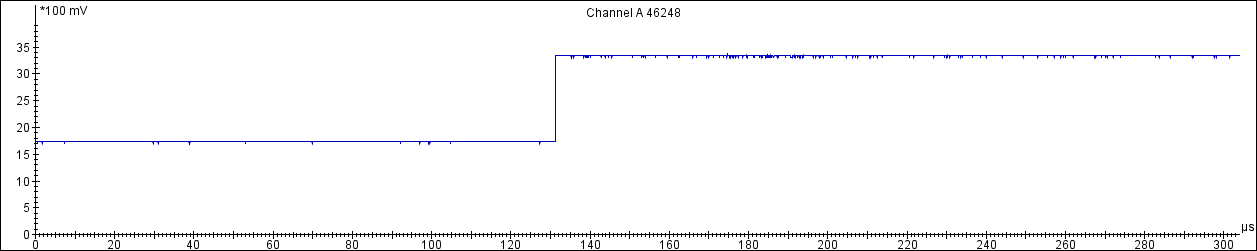
\includegraphics[width=\textwidth]{../plots/newplots/ti-trace-normal.png}
          }
          \subfigure[Normal-to-reset signal]{
            \label{fig:ti-error-traces-2}
            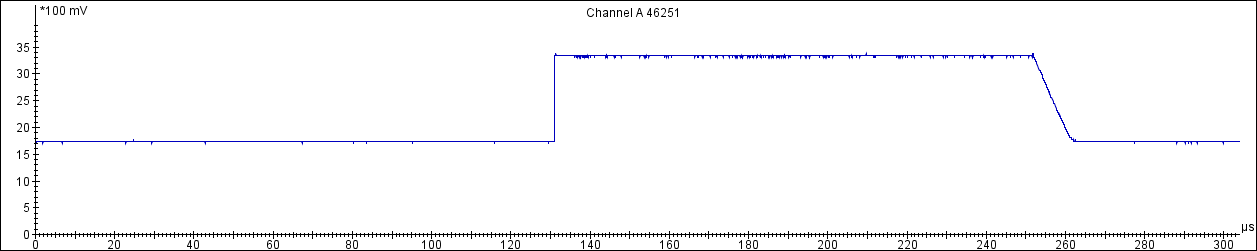
\includegraphics[width=\textwidth]{../plots/newplots/ti-trace-reset.png}
          }
          \subfigure[Fault detected signal]{
            \label{fig:ti-error-traces-3}
            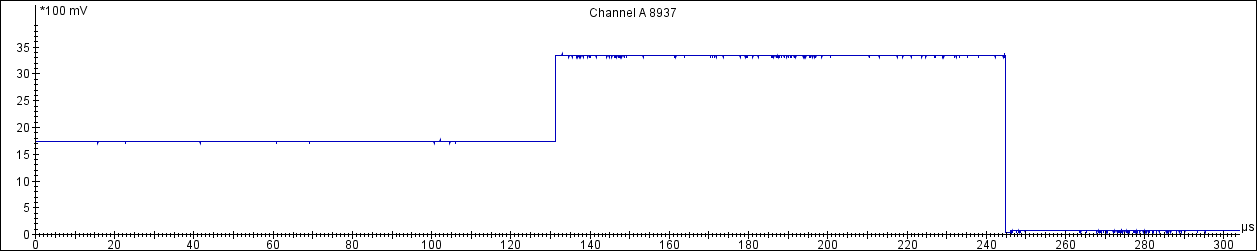
\includegraphics[width=\textwidth]{../plots/newplots/ti-trace-detected.png}
          }
          \caption{Different signals that can be observed on \errorpin}
          \label{fig:ti-error-traces}
      \end{figure}

      Before applying power glitches to the target, the development board has to be prepared. To combat minimal power supply fluctuations (noise), several capacitors are added to the board by the manufacturer. These have to be removed, in order to maximize the effect of a power glitch. These capacitors can be identified using the publicly available schematics \cite{texas_instruments_schematic} of the board. 
      Furthermore, it is desirable to isolate the power supply to the core as much as possible and to find a place to inject the glitch as close to the target as possible. The \TI has a number of separate power domains and the development board offers an easy access point to the core domain. This point is relatively far from the chip, as visible in \autoref{fig:ti-pic}, but is close enough as evidenced by the successful experiments.

      No special preparations to the target are required for EM glitching. In order to attempt to identify the specific system of the target on which the EM glitch as an effect, the layout of the chip can be investigated by removing the packaging of the chip with a 90\% nitric acid solution. %\todo{note that documentation of layout is typically secret?} 
      Applying this technique on the \TI and making pictures of the chip with a microscope results in the picture used in \autoref{fig:ti-unroll-x-y-ondie}.

      The JTAG debugging interface is protected by an `Advanced JTAG Security Module' (AJSM) \cite{texas_instruments_datasheet_2015}. By default the interface is unprotected and can be protected by writing a 128 bit value at address \texttt{0xF0000000} -- the password value. This address references a section of OTP memory, whose values can be changed from logical \texttt{1} to logical \texttt{0}. By setting at least one bit to \texttt{0}, the JTAG debugging interface can only be accessed by providing the right password value -- the bits that have been programmed -- to the ICEPick module that manages access to the debugging interface.
      
    \subsubsection{\ST }
    \label{sec:target-st}

      \begin{figure}[H]
        \centering
        \def\svgwidth{\columnwidth}
        \input{../pics/spc570-marked.pdf_tex}
        \caption{SPC570 location on the development board}
        \label{fig:fidiagram}
      \end{figure}

      This target implements a dual-core PowerPC e200z0h setup running at 80MHz. Similar to the \TI, the secondary CPU is running in lockstep configuration with the first. Unlike the \TI, other parts of the microcontroller, such as the interrupt handler, are running also in a separate lockstep configuration. Each of these replications feed into a local `Redundancy Control Checker Unit' (RCCU) and they in turn all provide input to a central system called the `Fault Collection and Control Unit' (FCCU), similar to the ESM in the \TI. This system also collects inputs from other fault handling systems offered by the target, such as error correction codes and cyclic redundancy checks. \cite{stmicroelectronics_datasheet_2015} Similar to the \TI, the FCCU system has several documented registers \cite{stmicroelectronics_technical_2015} available that provide information about which faults are detected and it offers a general output signal \errorpin that can be monitored. Unlike the \TI, this signal is provided through two separate signals -- \errorpinzero and \errorpinone -- and several protocols can be configured to indicate the state the microcontroller is in. By default, this protocol is the `Dual Rail' protocol. In this protocol a toggling differential signal should be observed during normal operation, as shown in \autoref{fig:st-error-traces-1}. When a fault is detected, both outputs toggle the same signal symmetrically, as pictured in \autoref{fig:st-error-traces-3}. During reset, no toggling is happening, as shown in \autoref{fig:st-error-traces-2}.

      \begin{figure}[H]
          \centering
          \subfigure[Normal signal]{
            \label{fig:st-error-traces-1}
            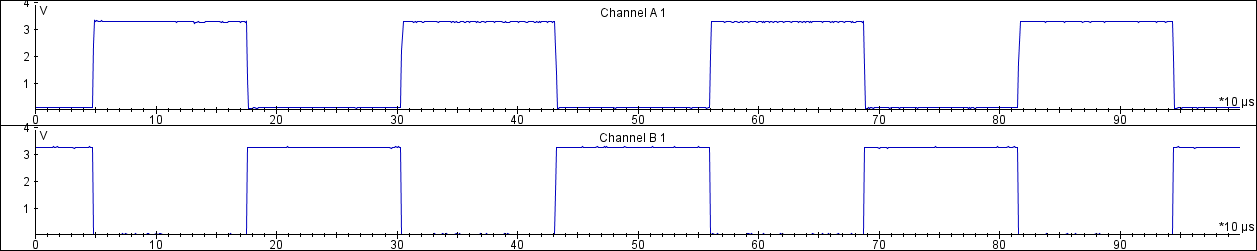
\includegraphics[width=\textwidth]{../plots/newplots/st-trace-normal.png}
          }
          \subfigure[Normal-to-reset signal]{
            \label{fig:st-error-traces-2}
            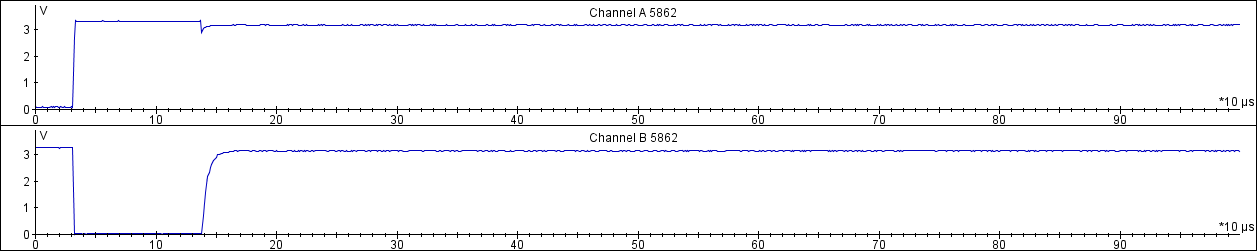
\includegraphics[width=\textwidth]{../plots/newplots/st-trace-reset.png}
          }
          \subfigure[Fault detected signal]{
            \label{fig:st-error-traces-3}
            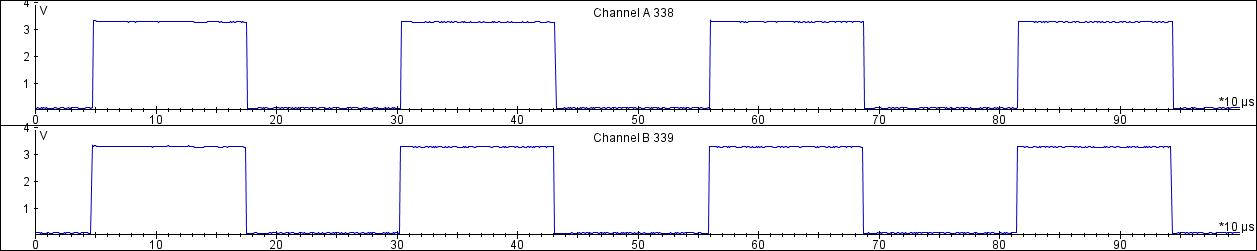
\includegraphics[width=\textwidth]{../plots/newplots/st-trace-detected.png}
          }
          \caption{different signals on error output}
          \label{fig:st-error-traces}
      \end{figure}


      \noindent Again similar to the \TI setup, measurements are categorized based on the state reported by the internal registers and the signal monitored on these two error output signals. 

      Also similar to the \TI, the development board was prepared for power glitching by removing all the external capacitors that are connected with the core power domain, consulting the schematics \cite{stmicroelectronics_schematic_2015}. In the preparatory phase it was also discovered that the 1.2V signal that powers the core cannot be directly provided externally (as is the case with the \TI) -- instead it can only be observed externally. The signal is generated from the 3.3V IO input voltage, by means of an internal voltage switching regulator, which brings the voltage down to 1.2V. The signal that this regulator produces is stabilized with the external capacitors. By removing too many of these capacitors, the signal becomes too noisy and the chip will no longer function. The recommended minimum capacitance that has to be added externally for the target to function properly is 1250nF \cite{stmicroelectronics_datasheet_2015} -- through trial-and-error the minimum amount of capacitance needed was found to be \textasciitilde56nF. The regulator is connected to the same power domain as the oscillator. The influence that the regulator has on power glitching is discussed in \autoref{sec:characterization-results}.


      Access to the JTAG debugging interface is managed by the `Password and Device Security Module' 
      \cite{stmicroelectronics_technical_2015}. This module manages the JTAG password, as well as a life cycle status register, censorship mode register, debug lock bit and several flash section lock registers. The values of these registers are taken from an OTP memory section called UTEST, which is filled with `Device configuration Format' (DCF) records. Depending on the life cycle state, censorship state, debug lock bit, a JTAG password value is required for accessing the interface. If an invalid password is provided, access to the JTAG interface is denied.

  \subsection{Glitching tools }
  \label{sec:hardwareused}
    This research has been performed in collaboration together with Riscure, who made both software and hardware available for this work to perform fault injection attacks \cite{riscure_hardware}: 

    \begin{description}
    \item[VC Glitcher] \ \\
    The VC Glitcher tool is central to both power glitching and EM glitching setups. It is configured by a host PC to generate glitches in a power supply line and pulses to control an EM glitch, all relative to a trigger. This trigger is input as a simple high low signal. It can generate glitches between -7.4V and +4.2V, with a precision of 2ns. And most importantly, all this is done in real-time.

    \item[Glitch Amplifier] \ \\
    The VC Glitcher might not be able to provide enough current for the device. By adding a Glitch Amplifier, up-to 1A of current can be provided.

    \item[EM Transient Probe] \ \\
    In the case of EM glitching, an EM Transient Probe is used to convert an input signal into an EM pulse. This pulse is generated with a changeable coil, allowing for customizability of orientation and width of the pulse. The maximum voltage that can be provided through the coil is 450V. 

    \item[XYZ Table] \ \\
    The EM probe is moved across the surface of the microcontroller using a mounting table that can move the probe three dimensions.

    \item[Current Probe] \ \\
    For current measurements a Current Probe has been added. It measures current by passing the to-be-observed power line through a coil, which is observed by a second coil.

    \item[icWaves] \ \\
    In the cases where a simple trigger signal is not available, the icWaves tool is used. This tool can monitor power signals and can be programmed  to generate a trigger when a reference pattern is observed. 

    \item[Inspector] \ \\
    All the aforementioned tools that require configuration and/or provide output are controlled by using the Inspector software tool.

    \item[pewpewplot] \ \\
    Results from measurements are plotted and analyzed by using the pewpewplot tool, which is a graphical front-end for the Python matplotlib package. All plots provided in this work are generated with this tool.

    \end{description}

    \noindent In addition to these in-house tools, some other devices have been used as well:

    \begin{description}
    \item[FTDI UART-USB cable] \ \\
    To monitor the fault that is caused by a glitch, simple serial protocols are used that can communicate with the host PC. 
    For these serial communications a generic FTDI UART-USB cable is used. 

    \item[PicoScope 5203] \ \\
    At various stages monitoring signals at different lines is necessary. In the basic cases, a multimeter can suffice. However, when more detailed information is required, an oscilloscope is required. Here the PicoScope 5203 has been used. 
    \end{description}

    \noindent Note that this equipment is fairly high end. With fault injection become more and more mainstream, cheaper solutions are also increasingly available. For example, solutions like \citet{chipwhisperer} are low cost solutions for fault injection utilizing power glitching.

  \subsection{Glitching setups }

    \begin{figure}[H]
      \centering
      \def\svgwidth{\columnwidth}
      \input{../pics/FIdiagram-power.pdf_tex}
      \caption{Power glitching setup}
      \label{fig:fidiagram-power}
    \end{figure}

    The tools mentioned in \autoref{sec:hardwareused} have been used in three different setups. The first, schematically shown in \autoref{fig:fidiagram-power}, uses the VC Glitcher to send a power glitch to the target. Responses are measured by transferring information of the internal state of the microcontroller with a simple serial protocol. 

    \begin{figure}[H]
    \centering
    \def\svgwidth{\columnwidth}
    \input{../pics/FIdiagram-EM.pdf_tex}
    \caption{EM glitching setup}
    \label{fig:fidiagram-em}
    \end{figure}

    \noindent The second setup uses the VC Glitcher to generate a signal which is converted into a high current spike by the EM Transient Probe, which is sent through a coil, generating a strong local electromagnetic field, which in turn results in a local current spike in the target. Responses are measured in a similar fashion as before, by transferring the internal state of the microcontroller over a serial line. This setup is schematically shown in \autoref{fig:fidiagram-em}. The EM Transient Probe is mounted on a table (not shown in the diagram) which can move the probe in all three dimensions. A photograph of how this setup comes together is given in \autoref{fig:ti-em-marked}. A close-up of the the EM probe positioned on top of the the target is shown in \autoref{fig:st-em}.

    \begin{figure}[H]
    \centering
    \def\svgwidth{\columnwidth}
    \input{../pics/FIdiagram-icWaves.pdf_tex}
    \caption{Glitching setup that does not rely on communication}
    \label{fig:fidiagram-icwaves}
    \end{figure}

    \noindent In the cases where (serial) output produced by the target is not enough to adequately trigger glitches and/or measure their effect, a third setup is used, shown in \autoref{fig:fidiagram-icwaves}. For triggering, the icWaves tool is used to observe an analog signal (e.g. the power consumption of the core). This signal is compared against a reference signal and produces a trigger signal for the VC Glitcher. To measure the effect of a glitch, a PicoScope is used to observe the same and/or different signals to aid in classifying measurements according to \autoref{tab:categories}. How all these parts come together in the example of power glitching is shown in \autoref{fig:ti-jtag-marked}.


    \begin{figure}[H]
      \centering
      \includegraphics[width=\textwidth]{../pics/photos/ti-st-marked.jpg}
      \caption{1: EM Transient Probe; 2: XYZ Table; 3: Host PC; 4: VC Glitcher}
      \label{fig:ti-em-marked}
    \end{figure}

    \begin{figure}[H]
      \centering
      \includegraphics[width=\textwidth]{../pics/photos/st-em.jpg}
      \caption{Close-up of the EM Transient Probe positioned atop the the target}
      \label{fig:st-em}
    \end{figure}

    \begin{figure}[H]
      \centering
      \includegraphics[width=\textwidth]{../pics/photos/ti-jtag-marked.jpg}
      \caption{1: icWaves; 2: Glitch Amplifier; 3: Target; 4: VC Glitcher; 5: PicoScope; 6: Host PC}
      \label{fig:ti-jtag-marked}
    \end{figure}

  \subsection{Attacking strategy } 
  \label{sec:attackstrategy}

    Two types of fault injection attacks have been performed: a set of characterization experiments, as outlined in \autoref{sec:characterization-explanation} and a more realistic JTAG attack as outlined in \autoref{sec:jtag-explanation}. In order to successfully inject a fault in a target, the parameters of the glitch that cause the fault have to be tuned -- this is discussed in \autoref{sec:parameters-tuning}. During the tuning of a glitch, multiple measurements are taken and classified. This is done using the categories described in \autoref{sec:classification}.

    \subsubsection{Characterization }
    \label{sec:characterization-explanation}

      The purpose of performing characterization experiments is to determine the sensitivity of a target to glitches and to find parameters for these glitches under which they cause a fault in a target in such a way that it displays the desired behavior. These experiments are done under full control of the attacker, which allows for the freedom to add triggers in software and read information of the state of the target from registers.
      Two such characterization experiments have been performed on the \TI and \ST. The first setup is named \unroll, the second is referred to as \auth. The setup for each of these experiment is explained below and the results of these experiments are presented and discussed in \autoref{sec:characterization-results}. A full table of the results can be found in \autoref{apdx:results} and their corresponding parameters in \autoref{apdx:parameters}. 
        \paragraph*{\unroll}  \ \\ \noindent
          In the \unroll experiment a very simple software is programmed on the target. The software raises a trigger, repeatedly performs the `add' instruction on a register and outputs the final value of the register:

          \begin{lstlisting}[label=lst:unroll, caption=Unroll experiment sample code]
            toggle_trigger();
            asm("add r4 #1");
            asm("add r4 #1");
            ... // repeat X-3 times
            asm("add r4 #1");
            toggle_trigger();
            send_r4_value();
          \end{lstlisting}

          \noindent The purpose of the \unroll experiment is to perform a very simple operation with as little variables as possible. To reduce the amount of variables, a clear window during which the glitch should be injected is signaled using some trigger signal -- for example, by raising a GPIO pin. Only one single instruction is repeatedly performed during this window, to minimize the effect of caches, pipelines, memory accesses and other CPU features that might influence the result of the glitch.

          The idea behind this experiment is to cause a fault in the \texttt{add} instruction in any way. The fault is deemed successful if the value that is sent after the execution differs from the \texttt{X} amount of times the instruction was performed. If the fault is unsuccessful, the expected value \texttt{X} is received. The expected value that is observed after a successful fault is \texttt{X-1}, which is caused by a fault affecting one \texttt{add} instruction in such a way that the register is not updated. However, many other values can be observed, for example by affecting the immediate being added.


      \paragraph*{\auth} \ \\ \noindent
        If the \unroll experiment is successful, a more realistic experiment should be performed. In this work, this is a simple conditional branch construction implemented with an \texttt{if}-statement. This setup simulates a simple flag check, which could indicate whether some authentication procedure has succeeded or not. This program looks like:

        \begin{lstlisting}[label=lst:auth, caption=Authentication experiment sample code]
          flag = 0;
          ...
          toggle_trigger();
          if (flag == 1)
            send_message("Authenticated!");
            led_on();
          else
            send_message("DENIED!");
          toggle_trigger();
        \end{lstlisting}

        \noindent Since this experiment is also performed in a very controlled environment, a trigger signal can again be added to indicate the window in which a fault should be injected. Note that due to the fact that this code is written in a higher level language, the compiler will likely introduce a number of additional instructions, depending on the amount of optimization, to load and store values from and to memory. A conditional branch such as \autoref{lst:auth} typically translates into a compare and a branch instruction. The added memory accesses make the setup more realistic than the \unroll experiment and might also make triggering mechanisms more likely.

        All the different instructions offer several places in which a fault can be effective. The compare instruction can be affected, possibly resulting in a compare flag that causes the branch instruction to execute the wrong branch. Or the branch instruction itself can be affected, causing the execution flow to simply go to sequentially the next piece of code -- in this case the wrong branch. A third option is affecting the flag value or the value against which it is being compared, resulting in a wrong input for the compare instruction. The exact effect does not matter much, as long as the wrong branch is executed, which is classified as a successful fault.

    \subsubsection{\jtag }
    \label{sec:jtag-explanation}

      The characterization experiments detailed in \autoref{sec:characterization-explanation} show whether glitches can cause successful faults in a target in general. 
      These experiments happen in an environment that is completely under the control of the attacker, allowing for customized output and trigger signals, making the experiments not a very realistic reflection of what would happen in a realistic setting. To show that a target is also breakable in a realistic setting, ideally the target would be found in a device used in the wild, for example an ECU. When this is not an option, for example due to unavailability, cost or for legal reasons, a good alternative is to attack the target's debugging interface. This debugging interface is typically implemented using the JTAG standard. Usually devices offer some way of locking this interface and attacking this locking mechanism should give a fair indication of the security of any implementations of the target found in the wild. Access to a debugging interface provides an attacker with the tools required for the attackers scenarios outlined in \autoref{sec:attacker-scenarios}. This is the final attack performed on one of the targets from \autoref{sec:targets}. This attack is referred to as \jtag henceforth. 

      The \jtag attack requires more investigatory work than the \unroll and \auth experiments. The mechanisms for locking devices vary widely from manufacturer to manufacturer and are often poorly documented. If documentation exists, it is typically proprietary and only shared upon signing a non-disclosure agreement. For the work presented here, only publicly available documentation has been used. \\

      \noindent The first thing to consider when trying to unlock the debugging interface is where a fault should be injected. The precise timing can be tuned through trial-and-error, but a rough window should be identified to keep the search space as small as possible. 
      A typical implementation of a JTAG protection scheme involves a section in memory where a password value can be programmed to. This value is then loaded into the system responsible for locking the JTAG interface. For more details on how this mechanism works exactly in the targets considered for this work, refer to \autoref{sec:targets}. 
      This value is read from memory every at every boot sequence and determines the actions that are performed during this sequence. The fact that different actions might occur offers an opportunity for profiling the target by recording power traces with different values programmed at this location, to identify a time frame where the fault should be injected. By analyzing the power consumption of an unlocked and locked target and comparing the two, differences might appear. 
      Another strategy to obtain this time frame is to program a different password value into the memory area for every boot sequence, to record the power consumption at every boot sequence and then to perform a correlation attack on the traces with the different password values. More details on the target specific side-channel analysis technique used and its results are given in \autoref{sec:realistic-attack}. 

      Note that for this profiling step, an attacker needs an exact copy of target over which he has full control --  for example by using a development board that has the target, as is done in this work. Profiling only needs to be done once and can then scale to all equal targets and possibly even similar targets. 

      The second thing to consider is that in order to inject the fault in the identified time frame, a reliable trigger signal is necessary. An attacker no longer has access to a user-defined trigger signal, as was the case during the characterization experiments. An easy alternative trigger signal is the power-on moment of a target. However, the time between the power-on moment and the point of interest is usually not time-constant, so this is not a good trigger signal if deterministic and repeatable faults are the purpose. A more complicated solution involves monitoring power consumption and using the patterns visible in the consumption as a trigger signal. This can be done with a tool such as icWaves \cite{riscure_hardware}. The experimental setup for this is schematically shown in \autoref{fig:fidiagram-icwaves}. 

      The final thing to consider is that output of the target is also not under control of the attacker. Determining whether a fault unlocked a device can tested by using debugging tools to, for example, read a section of the memory. But other categories, such as whether a reset occurred or if a fault was detected can not be determined this way. In order to make this distinction between reset and normal operation, power consumption can be monitored after injecting the fault. For differentiating between detected and undetected faults, the \errorpin signal can be monitored. \\

      \noindent In summary, the following steps are performed for the actual attack: 
      \begin{itemize}
        \item[]{\makebox[.75cm][l]{1.\hspace{.5cm}}inject glitch;}
        \item[]{\makebox[.75cm][l]{2.\hspace{.5cm}}match pattern in power consumption;}
        \item[]{\makebox[.75cm][l]{3.\hspace{.5cm}}generate trigger for setup;}
        \item[]{\makebox[.75cm][l]{4a.\hspace{.5cm}}monitor power consumption and other signals of the target;}
        \item[]{\makebox[.75cm][l]{\hspace{.15cm}b.\hspace{.5cm}}attempt to read or write memory via JTAG software.}
      \end{itemize}

    \subsubsection{Parameter tuning }
    \label{sec:parameters-tuning}
      Depending on the technique of glitching, different parameters can be tuned. 
      In the case of power glitching, the most parameters are: 
      \begin{itemize}
        \item the moment in time where glitch is injected (glitch offset); 
        \item the voltage of the voltage spike injected (glitch voltage); 
        \item and the length of the voltage spike (glitch length). 
      \end{itemize}
      \noindent Additionally, the number of glitches injected can be of importance and the base voltage supplied to the target can affect the results obtained \cite{massolino_smart_2015}.  
      For EM glitching the main parameters that have to be tuned are: 
      \begin{itemize}
        \item the glitch offset; 
        \item the position of the glitch in a 3 dimensional space (X, Y and Z coordinates); 
        \item and the strength of the glitch relative to the maximum glitch producible (glitch source power). 
      \end{itemize}
      \noindent Additionally, the number of glitches can be tuned as well. Furthermore, the polarity of the pulse and the area it affects can be configured manually. 

      Most of the time of a fault injection attack is spent on tuning these parameters to obtain a high number of successful faults. By consulting documentation and monitoring signals during normal operations, some of these parameters can be narrowed down to a relatively small window to reduce the search space, but fine-tuning still has to be performed after this. Typically a relatively broad set of values for each parameters is set to start experimentation with and through analysis of the results from these experiments, smaller windows are identified, eventually finding a single set of parameters with a high number of successful faults. This is the strategy applied in this work -- start by testing a broad set of values and then narrow these down to a single set. This is reflected in the parameter table in \autoref{apdx:parameters}.

      When a range of parameters are being tested, the most basic method is to randomly pick values from this range. More sophisticated methods of testing a range of parameters have been documented. For example, \citet{carpi_glitch_2013} compare the results of several methods of selecting and testing only sections in this range where successful faults are actually expected to occur. Such methods were not required to obtain the results presented in \autoref{sec:characterization-results} and \autoref{sec:realistic-attack}, so only basic random parameters selection has been used. Additionally, testing randomly selected parameter settings more closely approaches the safety setting than smarter methods of selection. 

    \subsubsection{Result classification }
    \label{sec:classification}


      After a set of glitching parameters is tested and measured, each measurement needs to be classified based on the observed effect. 
      In the experiments performed in this work, there are five categories of interest:
      \begin{enumerate}
        \item Glitches that did not have any observable effect and did not trigger any detection mechanism. These attempts are categorized as \UU (unsuccessful undetected). 
        \item Glitches that caused the target to reset, to stop responding or to stop working all-together. These attempts are categorized as \R (reset).
        \item Glitches that did not cause any observable effect, but did trigger the detection mechanism. These attempts are categorized as \UD (unsuccessful detected).
        \item Glitches that caused the desired effect, but were detected. These attempts are categorized as \SD (successful detected). 
        \item Glitches that caused the desired effect and went undetected. These attempts are categorized as \SU (successful undetected). 
      \end{enumerate}
      \begin{table}[H]
        \centering
        \begin{tabular}{llllc}
        \toprule
        & Category & ISO26262 & Color & Symbol \\%& Explanation  \\
        \midrule
        1. &\UU   & Safe & Green & $\blacksquare$ \\%& Glitch did not cause an observable fault, nor was it detected.  \\
        2. &\R    & Safe* & Yellow & \textbullet \\%& Glitch muted target or caused it to reset. \\
        3. &\UD   & Safe & Magenta & \texttimes \\%& Glitch did not cause an observable fault, but was detected.  \\
        4. &\SD   & Detected & Pink & + \\%& Glitch caused an observable fault, but was detected.  \\
        5. &\SU   & Residual & Red & $\blacklozenge$ \\%& Glitch caused an observable fault and was undetected.    \\
        \bottomrule
        \end{tabular}
        \caption{The categories used to classify the different effects of a glitch} 
        \label{tab:categories}
      \end{table}

      \noindent They are listed with the colors and symbols used to obtain the plots of the results sections in \autoref{tab:categories}. For comparison, the categories are mapped to the ISO26262 category which approximates the same definition, given the different context. Note that multiple-point faults are not considered in this work, as they were not required to obtain the results presented in \autoref{sec:characterization-results} and \autoref{sec:realistic-attack}. The categorization of \autoref{tab:categories} can easily be extended to include a similar mapping for these kinds of faults.

      In the simplest case, classification can be based on the register output produced by the target. When such output is not available, the classification can be based on more complicated signals, such as the power consumption of the core after a fault is injected or the \errorpin signals. This is previously discussed in \autoref{sec:targets}.

\newpage
\section{Characterization }
\label{sec:characterization-results}

  In this section the results of the characterization experiments discussed in \autoref{sec:characterization-explanation} that have been performed on the different targets mentioned in \autoref{sec:targets} are presented and discussed. \autoref{sec:characterization-overview} gives an overview of all the results in the form of a table and a discussion. \autoref{sec:effectiveness-countermeasures} covers the effectiveness of the mechanisms found in the targets. Finally, in \autoref{sec:characterization-observations} the effect that different parameters have on the successfulness of power glitches and EM glitches is investigated. 

  \subsection{Overview }
  \label{sec:characterization-overview}

    \begin{table}[H]
    \centering
    \begin{tabular}{l cc cc c }
    \toprule
             & \multicolumn{2}{c}{\unroll}  
      % \todo{is reset safe? unsuccessful didnt really cause any effect, so its nothing rather than safe?}
             & \multicolumn{2}{c}{\auth}        
             \\
               
               \cmidrule(lr){2-3}  \cmidrule(lr){4-5}  
             & \multicolumn{1}{c}{Power}                        & \multicolumn{1}{c}{EM}  
             & \multicolumn{1}{c}{Power}                        & \multicolumn{1}{c}{EM}                              
             \\
             \midrule
             \TI      
             & 87\%       %& \cellcolor{red!0}100\%     
             & 0.2\%      %& \cellcolor{red!0}100\%           
             & 60\%       %& \cellcolor{red!0}100\%    
             & 0.2\%      %& \cellcolor{red!0}100\%           
             \\
             \ST 
             & 0\% %& \cellcolor{green!0}\textasteriskcentered    
             & 19\%      %& \cellcolor{red!0}100\%    
             & \textasciitilde          %& \cellcolor{gray!0}  
             & 58\%       %& \cellcolor{red!0}100\%  
             \\
    \bottomrule
    \end{tabular}
    \caption{An overview of the success rates of the different characterization experiments under optimal parameter configurations} 
    \label{tab:experiments}
    \end{table}



    \autoref{tab:experiments} shows the success rates -- the amount of faults categorized as \SU -- of the two characterization experiments performed on the two targets. These percentages are obtained after tuning parameters to their approximate optimal settings. An optimal setting means that successful faults (\SU) are observed with the highest frequency, while no faults are reported by the detection mechanism, meaning no faults fall in the categories \SD and \UD. As discussed in \autoref{sec:attackstrategy}, these experiments are performed by starting with very broad settings for each of the parameters and by then narrowing these down to an optimal set of parameters.    
    The full results of the optimal configurations, as well as the results of the broader configurations can be found in \autoref{apdx:results}. The corresponding parameters are given in \autoref{apdx:parameters}.
    Both tables have four columns, corresponding to the `broadness' of the parameters used in that experiment, ranging from `Widest', which has very broad settings, to `Single' for which each parameter is set to a single fixed value. Note that not every experiment has been performed with four parameter settings. The reasons for this are that sometimes an optimal set of parameters could be found with less experimental steps (e.g., the `Wider' set of parameters already revealed enough information to find an  optimal `Single' set of parameters), or the \unroll experiment provided a more narrow starting point for the \auth experiment.

    The EM glitching on the \TI has a relatively low percentage of success. This is due to the fact that these experiments were only performed to confirm the sensitivity of the \TI to EM glitching for completeness sake. No time was spent to further narrow down optimal parameters, as these are already found for power glitching. 

    The power glitching on the \ST has a zero success rate. The reason for this is that the voltage regulator setup, addressed in \autoref{sec:target-st}, makes it non-trivial to inject a power glitch directly into the core. Several injection points have been tried: the 3.3V high voltage IO supply, the regulator power supply and the exposed output points of the 1.2V core voltage, all to no avail. The parameters and results of these experiments are separately included in \autoref{apdx:st-power}. Further investigation into a good place to inject a power glitch might prove successful, but due to the opportunity to use another glitching technique -- EM -- no further effort was spent on this.

    All the other experiments have a high enough success rate that successful faults can be injected into a target in a matter of seconds or minutes.


  \subsection{Effectiveness of mechanisms as countermeasures}
  \label{sec:effectiveness-countermeasures}

    In all of the characterization experiments it is possible to find parameters for which faults can be injected into the target a high amount of successful faults (category \SU), while these faults are never detected by the safety mechanisms (categories \SD and \UD). This is surprising, as all the experiments process data, which should give sufficient opportunity for either the lockstep mechanism or the error detection codes to detect discrepancies. A probable explanation for this result is that faults occur in some part of the system that is not covered by a safety mechanism. For example, a fault could be injected in a part of the system that is run in lockstep, effectively making both lockstep cores execute the same faulty instructions. Or the fault could affect the mechanism itself, preventing it from reporting its detection. The most likely explanation is that the fault affects the core in such a way that it does not produce behavior that is observable by the compare system.

    \subsubsection{\TI mechanisms } %\ \\

      The results obtained for the \TI can be used to further investigate which mechanisms are triggered, in the case a fault was detected. 
      For the parameters where detection was observed, some information on the kind of mechanisms that are triggered is reported by the registers of the fault detection mechanism in the \TI. Three experiments offer this opportunity -- \unroll with the widest parameter settings and \auth with wide (\authone) and less wide (\authtwo) parameter settings, performed with power glitching. These experiments report enough detected glitches to perform a meaningful analysis on them. Other experiments do not report detected faults, either because their parameters were tuned to a setting where no detected parameters were observed or an insignificant amount of faults were detected, as is the case with the EM experiments. \autoref{tab:tms570-unroll-auth-results} gives an overview of fault categorizations of these experiments.

      \begin{table}[H]
        \centering
        \begin{tabular}{l rr rr rr}
        \toprule

        & \multicolumn{2}{c}{\unroll}     &    
        \multicolumn{2}{c}{\authone}      &    
        \multicolumn{2}{c}{\authtwo}  \\
        \cmidrule(lr){2-3}                    
        \cmidrule(lr){4-5}
        \cmidrule(lr){6-7}
        \multicolumn{1}{c}{Category}  & 
        \multicolumn{1}{c}{Counts}      & \multicolumn{1}{r}{\%}          & 
        \multicolumn{1}{c}{Counts}      & \multicolumn{1}{r}{\%}          & 
        \multicolumn{1}{c}{Counts}      & \multicolumn{1}{r}{\%}          
        \\

        \midrule

        % \multicolumn{1}{c}{\multirow{3}{*}{ \parbox{2cm}{\TI power \unroll}}}

        \UU    
        & 60048  & 38.26\%                   
        & 33669   & 19.83\%                     
        &  73543  & 43.82\%                 
        \\
        \R   
        & 57436  & 36.60\%                   
        & 106323  & 62.62\%                     
        &  50751  & 30.24\%                 
        \\
        \UD  
        & 15711  & 10.01\%                   
        & 26877   & 15.83\%                     
        &  32265  & 19.22\%                 
        \\
        \SD     
        & 22610  & 14.40\%                   
        & 2806    & 1.652\%                     
        &  10049  & 5.988\%                 
        \\
        \SU      
        & 1107   & 0.705\%                   
        & 94      & 0.055\%                     
        &  1200   & 0.715\%                 
        \\

        \cmidrule(l){1-7}
        total    
        & 156912 &                            
        & 169769  &                           
        &  167808 &                               
        \\       


        \bottomrule
        \end{tabular}
        \caption{\TI \unroll and \auth}
      \label{tab:tms570-unroll-auth-results}
      \end{table}

      \paragraph*{\unroll vs. \auth } \ \\ \noindent
        \autoref{tab:tms570-fault-overview-auth-unroll} shows the amount of times a certain fault was detected by a mechanism and how many of the total amount of detected (\UD and \SD combined) faults -- 38321 (24\% of the faults), 29683 (17\%) and 42314 (25\%) respectively -- they are. 
        In \unroll 1107 (0.7\%) faults are successful and undetected (\SU), while in \auth this is the case for 94 (0.6\%) for the wider parameters settings and 1200 (0.7\%) for the narrower parameter settings of the faults. For \authone and \authtwo an additional column is added to \autoref{tab:tms570-fault-overview-auth-unroll} that indicates the increase or decrease in detections of that fault, relative to \unroll. Note that in each measurement multiple mechanisms can be triggered.

        All mechanisms are investigated through the registers that are exposed by the `Error Signaling Module' (ESM). Mechanisms are grouped together, and each group has its own register(s). In addition to these registers, the \errorpin has its own register, which is also monitored and the `CPU Compare Module for Cortex-R4F' (CCM-R4F) exposes a register that allows to investigate the state of the lockstep mechanism -- `CCM self test error' in this table.
     
        % \newgeometry{left=0cm,right=0cm}
        \begin{table}[H]
          \centering
          \begin{tabular}{lr|rr|rr}
          \toprule
          \multicolumn{1}{c}{\ }
          & \multicolumn{1}{c}{\unroll}
          & \multicolumn{2}{c}{\authone}
          & \multicolumn{2}{c}{\authtwo}
          \\
          \cmidrule(lr){2-2}  
          \cmidrule(lr){3-4}  
          \cmidrule(lr){5-6}  
          Fault signaled
          & \multicolumn{1}{c}{\%} 
          & \multicolumn{1}{c}{\%} & \multicolumn{1}{c}{$\Delta$} & \multicolumn{1}{c}{\%} & \multicolumn{1}{c}{$\Delta$}
          \\
          \midrule
          cpu compare error 
          & 99.89\%
          & 99.42\% & -0.48\%
          & 99.92\% & +0.03\%
          \\
          error pin raised 
          & 99.04\%
          & 85.80\% & -13.25\%
          & 92.34\% & -6.70\%
          \\
          lockstep error 
          & 98.22\%
          & 84.78\% & -13.44\%
          & 92.29\% & -5.93\%
          \\
          CCM self test error 
          & 98.01\%
          & 84.69\% & -13.32\%
          & 92.29\% & -5.72\%
          \\
          % dmagroup & interrupts
          % & 32.94\%
          % & 0.00\% & -32.94\%
          % & 0.00\% & -32.94\%
          % \\
          flash address parity error% in flash 
          % FMC address parity error flash 
          & 27.08\%
          & 18.16\% & -8.92\%
          & 12.31\% & -14.77\%
          \\
          RAM parity error 
          % DMA RAM parity error & ESMSR1
          & 21.54\%
          & 19.93\% & -1.61\%
          & 25.75\% & +4.20\%
          \\
          ECC error in OTP 
          % FMC ECC error in OTP 
          & 2.55\%
          & 2.24\% & -0.31\%
          & 5.44\% & +2.89\%
          \\
          % VIM RAM parity error & ESMSR1
          % & 1.39\%
          % & 0.00\% & -1.39\%
          % & 0.00\% & -1.39\%
          % \\
          % PLL\#2 slip & ESMSR4
          % & 0.49\%
          % & 0.73\% & +0.25\%
          % & 0.00\% & -0.49\%
          % \\
          % B1TCM address bus parity error 
          % & 0.01\%
          % & 0.35\% & +0.35\%
          % & 0.03\% & +0.02\%
          % \\
          RAM ECC error 
          % B1TCM RAM ECC error & ESMSR3
          & 0.00\%
          & 1.55\% & +1.54\%
          & 1.01\% & +1.01\%
          \\
          % esm1 & interrupts
          % & 0.00\%
          % & 0.00\% & -0.00\%
          % & 0.00\% & -0.00\%
          % \\
          eFuse controller error 
          & 0.00\%
          & 3.14\% & +3.14\%
          & 0.26\% & +0.26\%
          \\
          undocumented channel 
          & 0.00\%
          & 3.14\% & +3.14\%
          & 0.26\% & +0.26\%
          \\
          clock compare error 
          & 0.00\%
          & 3.14\% & +3.14\%
          & 0.26\% & +0.26\%
          \\
          power domain error 
          % power domain controller error 
          & 0.00\%
          & 3.13\% & +3.13\%
          & 0.26\% & +0.26\%
          \\
          %     B0TCM correctable ECC error & ESMSR1
          % & 0.00\%
          % & 0.48\% & +0.48\%
          % & 0.00\% & +0.00\%
          % \\
          % esm2 & interrupts
          % & 0.00\%
          % & 0.12\% & +0.12\%
          % & 0.00\% & +0.00\%
          % \\
          % B0TCM address bus parity error 
          % & 0.00\%
          % & 0.09\% & +0.09\%
          % & 0.00\% & +0.00\%
          % \\
          % B0TCM RAM ECC error & ESMSR3
          % & 0.00\%
          % & 0.01\% & +0.01\%
          % & 0.00\% & +0.00\%
          % \\
          % B0TCM RAM address decode error 
          % & 0.00\%
          % & 0.01\% & +0.01\%
          % & 0.00\% & +0.00\%
          % \\
          % sci & interrupts
          % & 0.00\%
          % & 0.00\% & +0.00\%
          % & 0.00\% & +0.00\%
          % \\
          % mystery register on & ESMG1 ???
          % & 0.00\%
          % & 0.00\% & +0.00\%
          % & 0.00\% & +0.00\%
          % \\
          % B1TCM RAM address decode error 
          % & 0.00\%
          % & 0.00\% & +0.00\%
          % & 0.00\% & +0.00\%
          % \\
          \bottomrule
          \end{tabular}
        \caption{Percentages of triggered safety mechanisms for three different experiments, of which the latter two are compared with the first}
        \label{tab:tms570-fault-overview-auth-unroll}
        \end{table}
        % \restoregeometry

        \autoref{tab:tms570-fault-overview-auth-unroll} shows that by far the most effective measure is the lockstep mechanism, as in all experiments it is (partly) responsible for $>$99\% of the detections. Interestingly, not all faults detected in the CCM reach the ESM, meaning that it was reported in the CCM register, but did not result in an assertion of the \errorpin signal. This happens the most in the \authone experiment -- here \textasciitilde14\% of the detected faults do not result in either a lockstep error or CCM self test error in the ESM and consequently do not raise the \errorpin signal, as illustrated by \autoref{tab:tms570-unroll-auth-errorpinvslockstep}. 

        \begin{table}[H]
          \centering
          \begin{tabular}{p{.5cm}p{.5cm}rrrrrr}
          \toprule

          &
          & \multicolumn{2}{c}{\unroll}
          & \multicolumn{2}{c}{\authone}
          & \multicolumn{2}{c}{\authtwo}
          \\
          \cmidrule(lr){3-4}  
          \cmidrule(lr){5-6}  
          \cmidrule(lr){7-8}  
          cce & epr
          & Count & \%  & Count & \%  & Count & \%
          \\
          \midrule
          \texttimes& \texttimes &
          37955 & 99.04\%
          & 25316 & 85.29\%
          & 39044 & 92.27\%
          \\
          \texttimes&  &
          325 & 0.85\%
          & 4194 & 14.13\%
          & 3238 & 7.65\%
          \\
          &\texttimes&  
          0 & 0.00\%
          & 0 & 0.00\%
          & 0 & 0.00\%
          \\
          &  &
          41 & 0.11\%
          & 22 & 0.07\%
          & 2 & 0.00\%
          \\
          \bottomrule
          \end{tabular}
        \caption{A comparison amount of times a certain combination of cpu compare error (cce) and error pin raised (epr) was observed}
        \label{tab:tms570-unroll-auth-errorpinvslockstep}
        \end{table}

        \noindent In \authtwo this discrepancy drops to \textasciitilde8\% and in  \unroll this amount is $<$1\%. The inconsistency in faults detected by the CCM and faults detections that reach the ESM means that implementations that rely only on the ESM, either on the interrupts it can generate or on the \errorpin signal it can assert (the recommended method of handling faults), a significant amount of detected lockstep faults will be missed.

        Note that both the `lockstep error' and `CCM self test error' channels are used to report a fault detected by the lockstep mechanism in the CCM. This provides a second redundant channel over which the lockstep mechanism can report faults to the ESM. The results show that this slightly helps in the faults detection propagation, as in both experiments a small amount ($<$1\%) of the detected faults were not signaled over both channels. 

        For \unroll, the most effective ECDC mechanisms are the parity checks performed on addresses in flash and parity checks in the RAM, with the first having the most impact. This is also the case for \authone, but here both measures amount in a similar amount of detections. In \authtwo, RAM parity checks are significantly more effective than any other ECDC measure, including the parity checks performed on addresses in flash. \authtwo has a fairly specific point in time in which a fault is injected, which can explain the fact that more specific mechanisms are triggered.

        Furthermore, a slightly broader range of fault detection mechanisms are triggered in the \auth experiments. This can be caused by the fact that the software that runs on the target during the \auth experiments performs more different instructions, which allows for a broader range of ways a fault can influence the execution. Finally, in the results of the \auth experiments a number of fault channels reports faults that are not documented in the datasheet, summarized under `undocumented channel' in \autoref{tab:tms570-fault-overview-auth-unroll}. 


      \paragraph*{\UD vs \SD} \ \\ \noindent
        Comparing detected faults between the two types of detected faults -- \UD and \SD -- reveals that the \SD results show less variety in the different types of the mechanisms triggered and also shows a increase in the amount of lockstep detected faults that are successfully propagated to the ESM. This effect is illustrated in \autoref{tab:tms570-fault-overview-auth-ud-sd} which shows the results of \authone separated by category. Other experiments show the same differences between both categories.

        \begin{table}[H]
          \centering
          \begin{tabular}{lr|rr}
          \toprule
          \multicolumn{1}{c}{\ }
          & \multicolumn{1}{c}{\authone \UD}
          & \multicolumn{2}{c}{\authone \SD}
          \\
          \cmidrule(lr){2-2}  
          \cmidrule(lr){3-4}  
          Fault signaled
          & \multicolumn{1}{c}{\%} 
          & \multicolumn{1}{c}{\%} & \multicolumn{1}{c}{$\Delta$}
          \\
          \midrule
          cpu compare error 
          & 99.38\%
          & 99.79\% & +0.41\%
          \\
          error pin raised 
          & 85.01\%
          & 93.37\% & +8.37\%
          \\
          lockstep error 
          & 83.94\%
          & 92.80\% & +8.86\%
          \\
          CCM self test error 
          & 83.86\%
          & 92.66\% & +8.80\%
          \\
          RAM parity error 
          % DMA RAM parity error 
          & 19.37\%
          & 25.30\% & +5.93\%
          \\
          flash address parity error 
          & 18.12\%
          & 18.53\% & +0.41\%
          \\
          undocumented channel 
          & 3.47\%
          & 0.04\% & -3.43\%
          \\
          clock compare error 
          & 3.47\%
          & 0.04\% & -3.43\%
          \\
          eFuse controller error 
          & 3.47\%
          & 0.04\% & -3.43\%
          \\
          power domain controller error 
          & 3.46\%
          & 0.00\% & -3.46\%
          \\
          ECC error in OTP 
          & 2.31\%
          & 1.53\% & -0.78\%
          \\
          % B1TCM RAM ECC error & ESMSR3
          % & 1.54\%
          % & 1.57\% & +0.02\%
          % \\
          % PLL\#2 slip & ESMSR4
          % & 0.73\%
          % & 0.82\% & +0.09\%
          % \\
          % B0TCM correctable ECC error & ESMSR1
          % & 0.50\%
          % & 0.25\% & -0.25\%
          % \\
          % B1TCM address bus parity error & ESMSR2
          % & 0.32\%
          % & 0.68\% & +0.36\%
          % \\
          % esm2 & interrupts
          % & 0.13\%
          % & 0.00\% & -0.13\%
          % \\
          % B0TCM address bus parity error & ESMSR2
          % & 0.10\%
          % & 0.00\% & -0.10\%
          % \\
          % B0TCM RAM ECC error & ESMSR3
          % & 0.01\%
          % & 0.00\% & -0.01\%
          % \\
          % B0TCM RAM address decode error & ESMSR2
          % & 0.01\%
          % & 0.00\% & -0.01\%
          % \\
          % B1TCM RAM address decode error & ESMSR2
          % & 0.00\%
          % & 0.00\% & -0.00\%
          % \\
          % mystery register on & ESMG1 ???
          % & 0.00\%
          % & 0.00\% & -0.00\%
          % \\
          % sci & interrupts
          % & 0.00\%
          % & 0.04\% & +0.04\%
          % \\
          \bottomrule
          \end{tabular}
        \caption{Percentages of triggered safety mechanisms in the \authone experiment, separated in categories \SD and \UD}
        \label{tab:tms570-fault-overview-auth-ud-sd}
        \end{table}

        The experiments also show that in the \SD category a higher amount of RAM parity errors is detected. Additionally, in the case of \authtwo -- the experiment with the least wide parameter settings -- a strong drop in amount of faults detected by parity checks performed on addresses in flash is observed. 

        In the measurements that are categorized as \SD category, faults have an observable effect on the computation, contrary to the category of \UD, where no observable effect is present. This difference is a possible explanation for the increase in memory based mechanisms that are triggered.

    \subsubsection{\ST mechanisms }% \ \\
        The \ST does not report any faults through the registers that are sent over serial and as such does not allow for an investigation similar to the one done on the \TI, despite careful configuration of the microcontroller. Moreover, by investigating the error output pins in a setup like \autoref{fig:fidiagram-icwaves}, the microcontroller never enters a fault detected state, meaning that the \errorpin signals never go into the error detected state shown in \autoref{fig:st-error-traces} -- only the normal and reset patterns are observed. Investigation of the \errorpin signals does reveal that two different types of reset occur. In the first, the target actually resets. In the second, the target does not output any serial output, but the error reporting pins remain in the normal state (the target was muted).

        A possible explanation for the fact that no registers showed any errors, is that the fault detection mechanism immediately resets after a fault is detected. However, this is not a problem, as successful faults are still achievable with comfortable percentages, as shown in \autoref{tab:experiments}.

  \subsection{Analysis of parameters }
  \label{sec:characterization-observations}
    The different parameters that can be tuned for a glitch typically all have a profound effect on the rate 
    of successful faults. Additionally many parameters show some relationship to one another. These observations can be made independent of the target on which they are performed, which is why they are listed in this section per parameter, rather than per target. Each observation is supported by one or more examples from the experiments performed. The meaning of the colors and symbols in the plots shown can be found in \autoref{tab:categories}. 

    \paragraph*{Glitch offset }
        The offset of a glitch relative to its trigger is very influential to the success rate of a glitch, for both power and EM glitches. This shows the importance of the temporal aspect of a fault that a glitch causes. In the \unroll experiments, this is visible by a periodicity in the successful faults, indicating that different \texttt{add} instructions are affected as shown \autoref{fig:ti-unroll-offset-length}. In the \auth experiment this is apparent by a sharp cut-off point, after which faults are no longer successful.

        \begin{figure}[H]
          \centering
          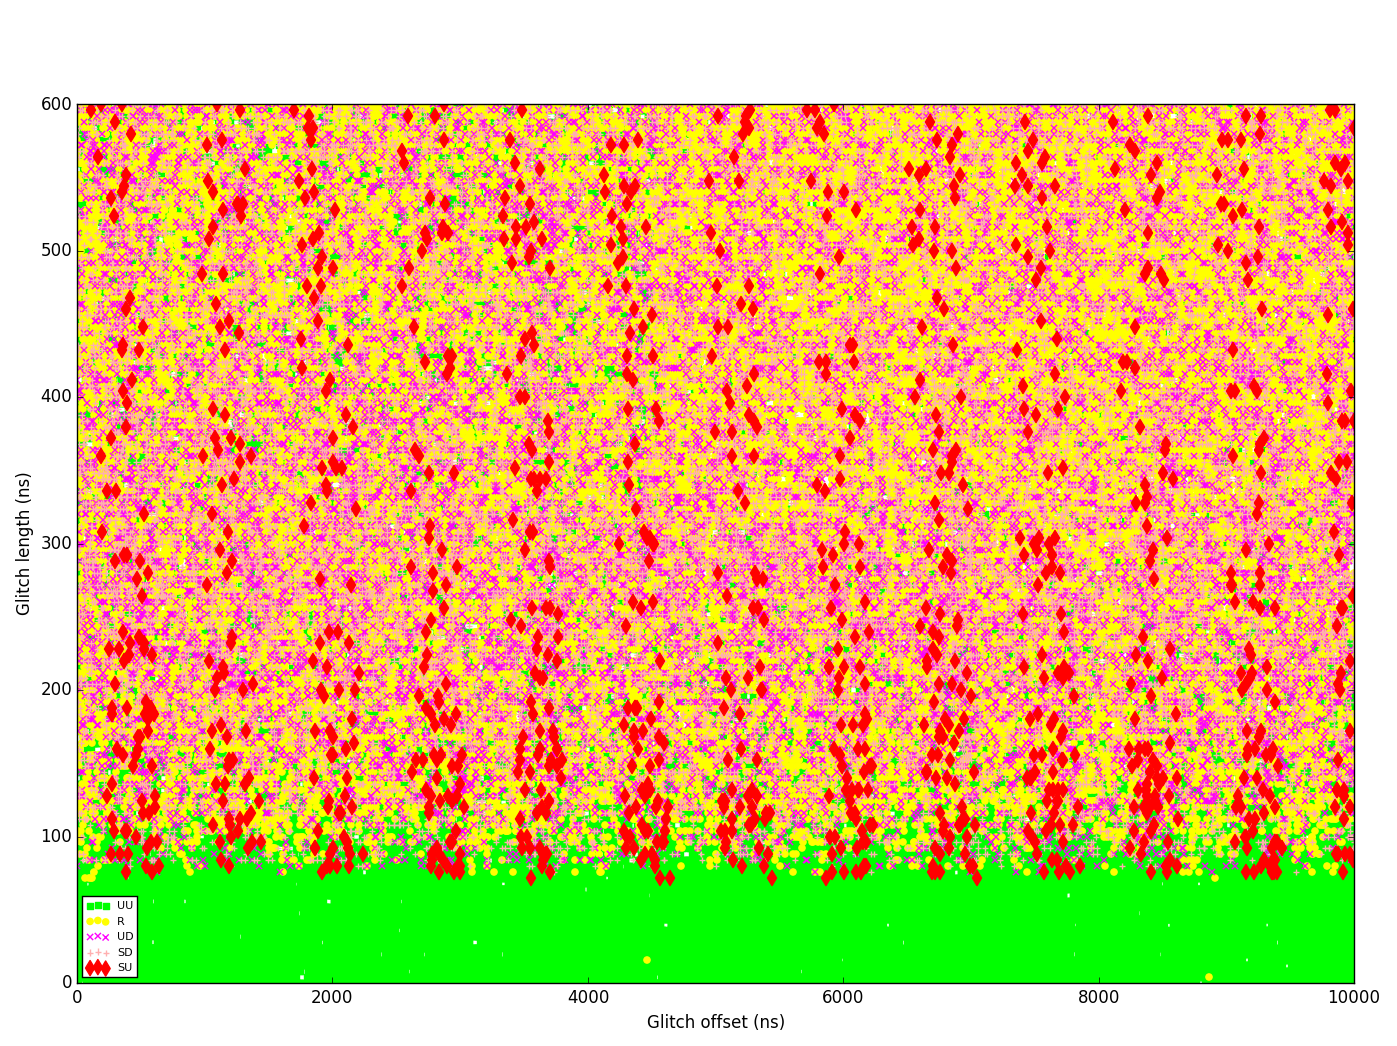
\includegraphics[width=\textwidth]{../plots/newplots/ti-unroll-offset-length.png}
          \caption{\TI \unroll glitch offset vs. length}
          \label{fig:ti-unroll-offset-length}
        \end{figure}

    \subsubsection{Power glitching parameters}

      \paragraph*{Glitch length and glitch voltage}% \ \\
        Glitch voltage and glitch length determine the `strength' of a power glitch. The effect of the strength of a glitch on the success rate of a fault can be investigated by plotting them together -- this reveals two areas that have a boundary of a typical \cite{carpi_glitch_2013} shape. The two areas show a separation of two categories: the glitches that cause a reset (\R category) and the glitches that do not have any effect (\UU category). The boundary is where most of the glitches with a desirable fault are observed (the \SD and \SU categories). This is also the case for the \TI, as shown in \autoref{fig:ti-unroll-voltage-length}. The reason for this shape is that, even after removing all the external capacitance of a target, the internal capacitance is still significant enough to slightly filter the the glitch signal. This can be overcome by either increasing the glitch voltage or the glitch length, or by increasing both, resulting in the shape visible.

        During the JTAG attack discussed later in \autoref{sec:realistic-attack}, a different shape appears in the glitch length and glitch voltage relationship. Typically a single curved boundary between the \UU and \R categories is visible, as seen in \autoref{fig:ti-unroll-voltage-length}. However, in \autoref{fig:ti-jtag-voltage-length} a second boundary seems to appear. The exact reason for this is hard to determine, possible explanations are that the lockstep core shows a different characteristic, or perhaps a different sensitive system is affected. Inspection of the \errorpin signal shows that the peculiar shape is not caused by a difference between glitches that caused a mute and caused a reset that resides in this category.

        \begin{figure}[H]
          \centering
          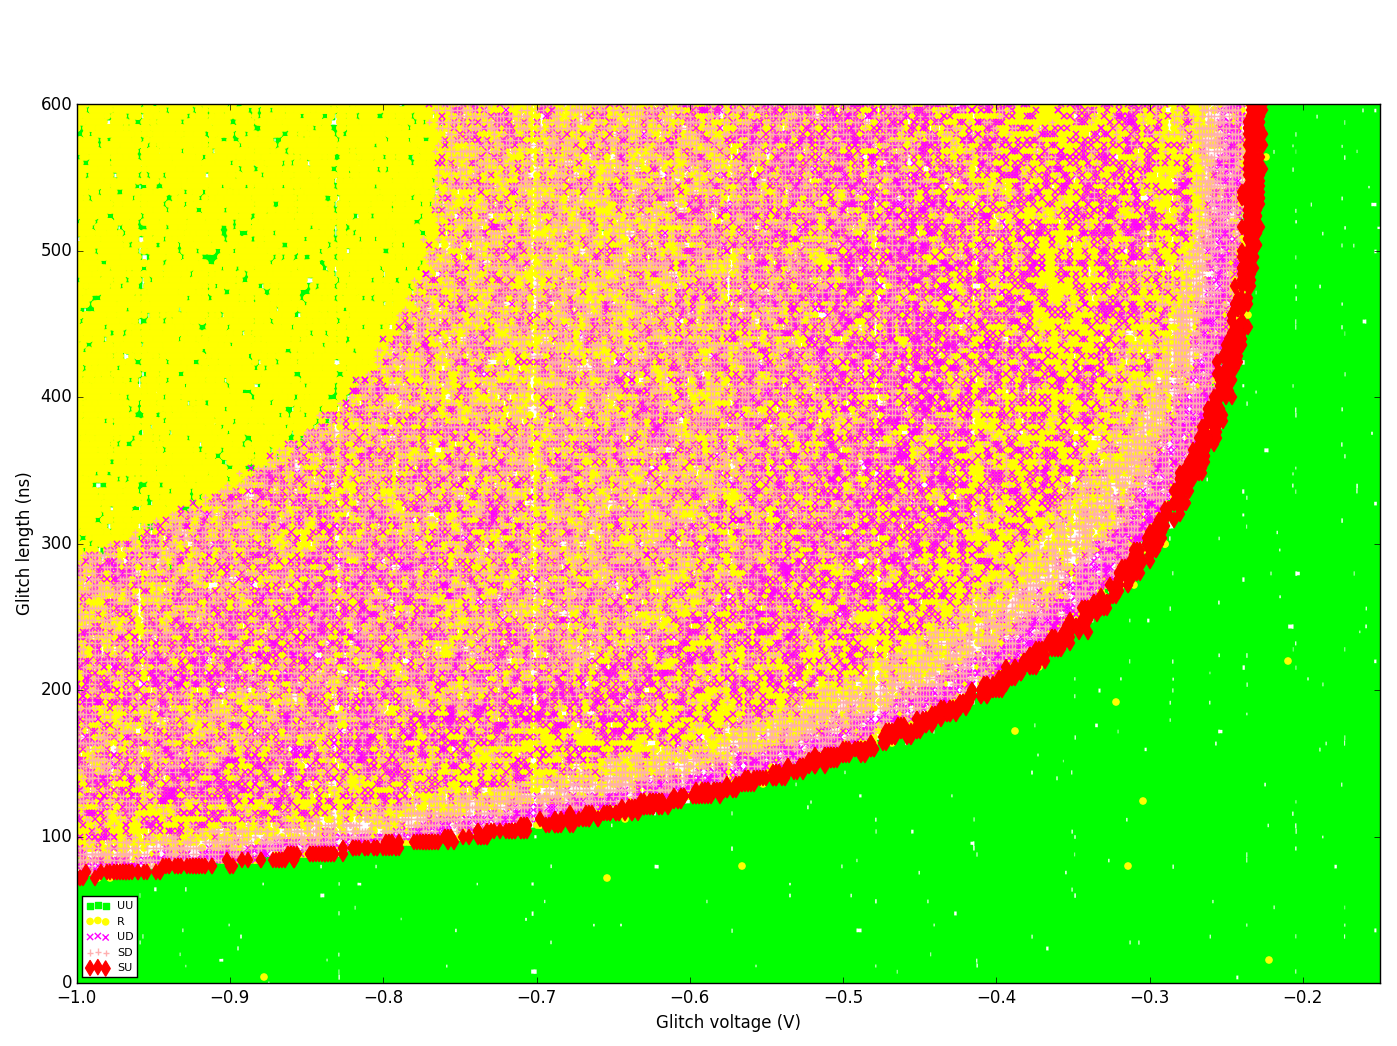
\includegraphics[width=\textwidth]{../plots/newplots/ti-unroll-voltage-length.png}
          \caption{\TI \unroll glitch voltage vs. length}
          \label{fig:ti-unroll-voltage-length}
        \end{figure}

        \paragraph*{Glitch offset and glitch `strength'} %\ \\
          The glitch strength that defines the shape of a glitch and the glitch offset are also highly dependent on each other. This effect is harder to visualize in a two dimensional plot, as it is determined by three separate parameters. By binning measurements based on the offset, this effect becomes apparent, as shown in \autoref{fig:ti-auth-voltage-length-offsets}. The successful faults -- both detected and undetected -- appear to move along the boundary from weaker glitch parameters to stronger parameters as offset values increase, meaning that the glitch is injected closer to the point of success.

          \begin{figure}[H]
            \centering
            \subfigure[Glitch offset between 30849ns and 30890ns]{
              \label{fig:ti-auth-voltage-length-offsets-1}
              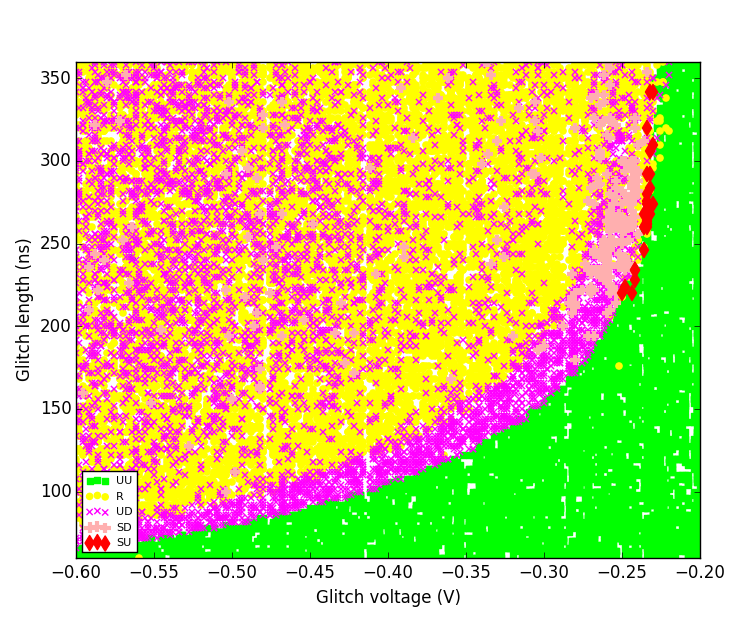
\includegraphics[width=.45\textwidth]{../plots/newplots/ti-auth-voltage-length-offets-1.png}
            }
            ~
            \subfigure[Glitch offset between 30891ns and 30930ns]{
              \label{fig:ti-auth-voltage-length-offsets-2}
              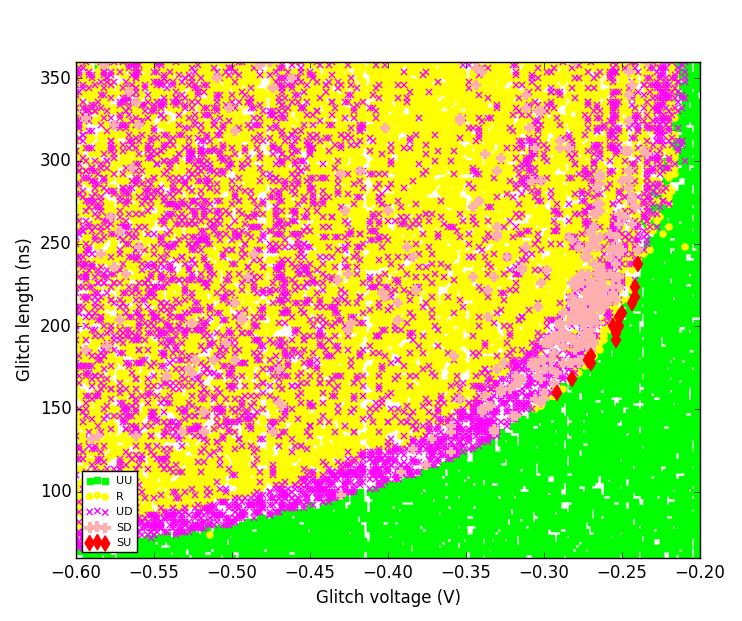
\includegraphics[width=.45\textwidth]{../plots/newplots/ti-auth-voltage-length-offets-2.png}
            }
            \\
            \subfigure[Glitch offset between 30931ns and 30970ns]{
              \label{fig:ti-auth-voltage-length-offsets-3}
              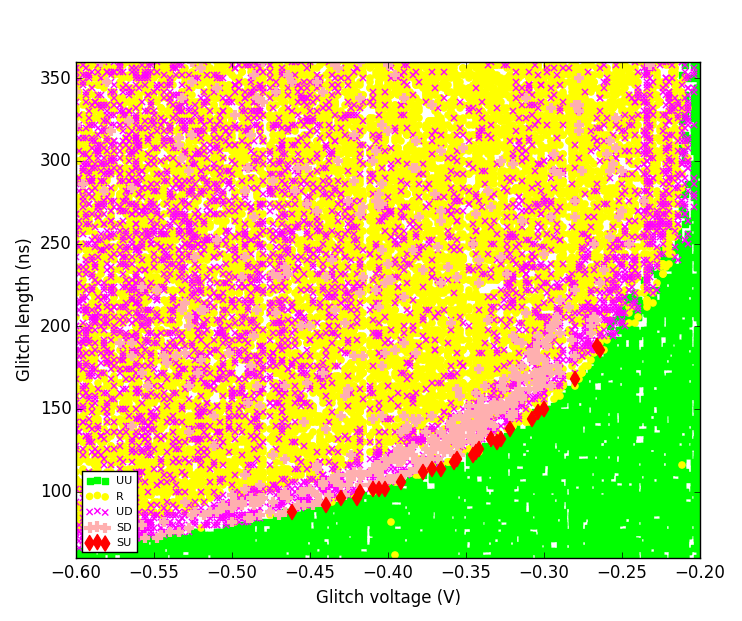
\includegraphics[width=.45\textwidth]{../plots/newplots/ti-auth-voltage-length-offets-3.png}
            }
            ~
            \subfigure[Glitch offset between 30971ns and 31100ns]{
              \label{fig:ti-auth-voltage-length-offsets-4}
              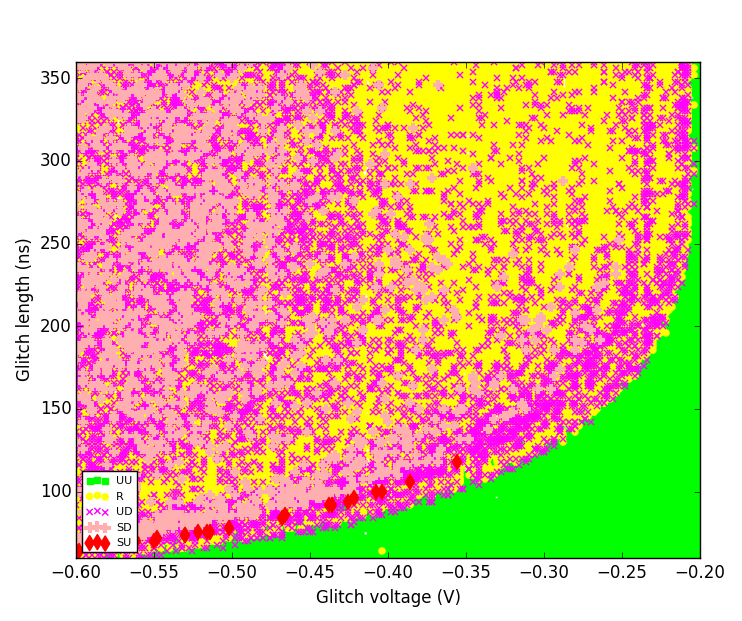
\includegraphics[width=.45\textwidth]{../plots/newplots/ti-auth-voltage-length-offets-4.png}
            }
            \caption{Glitch voltage vs. glitch length, binned in groups of glitch offset \TI power \auth}
            \label{fig:ti-auth-voltage-length-offsets}
          \end{figure}

          \noindent As mentioned before, a power glitch has to reach a certain threshold value to cause a certain successful fault. Due to factors such as internal capacitance, voltage drops do not reach this threshold instantly -- instead, a stronger glitch voltage reaches this threshold faster while a weaker glitch voltage reaches this threshold later in time. A very simplified illustration of this effect is shown in \autoref{fig:slopdiagram}, with some example parameters. Voltage threshold \textsc{t} needs to be reached at point \textsc{p} in time for a successful fault.

          \begin{figure}[H]
            \centering
            \def\svgwidth{\columnwidth}
            \input{../pics/slope-diagram.pdf_tex}
            \caption{Schematic representation of the effects that glitch length, glitch voltage and glitch offset have on reaching required power threshold \textsc{T} at required moment in time \textsc{P}}
            \label{fig:slopdiagram}
          \end{figure}

      % \end{description}

    \subsubsection{EM glitching parameters }

      % \begin{description}
      \paragraph*{X and Y position}
        The EM experiments on both targets confirm that the spatial component of an EM glitch has a strong effect on the rate of obtaining a successful fault, as shown by each of the plots shown in the collective \autoref{fig:st-unroll-x-y-offsets}. In these plots there are clear areas visible on the surface of the chip where a glitch has an effect (e.g. any category besides \UU), and other areas where nothing happens (categorized as \UU). These plots also show that there is a broad area where glitches cause a successful undetected fault. This indicates that there are systems inside the chip that, when targeted by an EM glitch, cause a successful fault.

        The experiments performed on the \TI show an additional interesting point -- whether a fault is detected or not also depends on the spatial parameter of the glitch. This shows that it is possible to specifically hit mechanisms, or avoid them entirely. 
        This is shown in \autoref{fig:ti-unroll-x-y-ondie}, where the measurements of an already narrowed down measurement are plotted on top of a picture of the chip that is found after removing the packaging, using the process described in \autoref{sec:target-ti}.

        \begin{figure}[H]
          \centering
          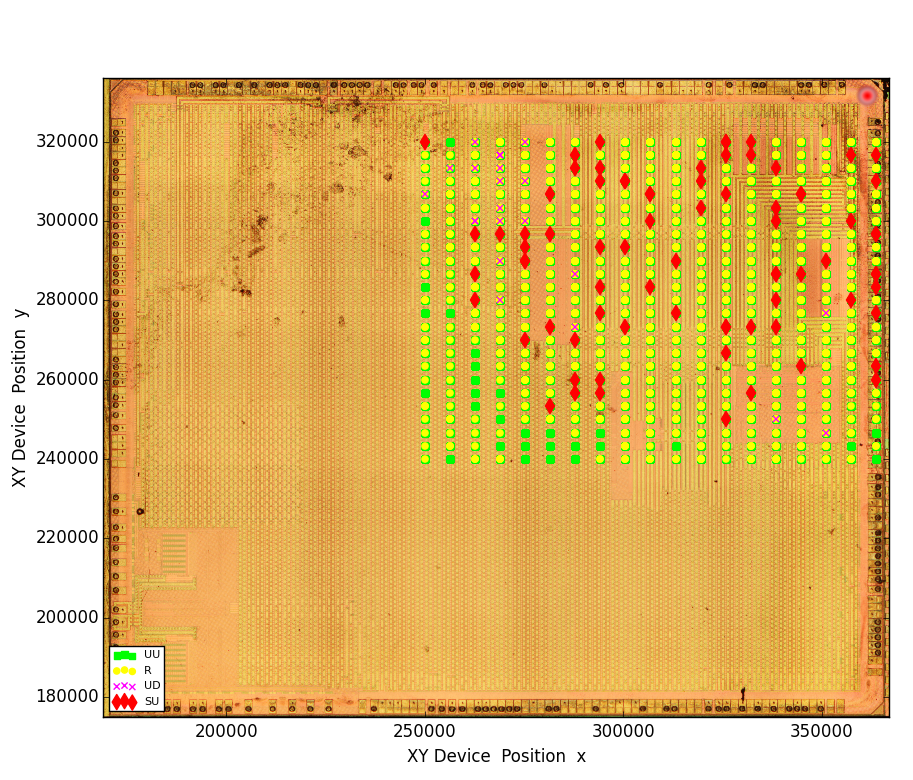
\includegraphics[width=\textwidth]{../plots/newplots/ti-auth-x-y-ondie.png}
          \caption{\TI \unroll glitch voltage vs. length}
          \label{fig:ti-unroll-x-y-ondie}
        \end{figure}

      \paragraph*{Glitch source power}
        The power of an EM glitch has a profound effect on the area of the chip that is affected. A weaker glitch will induce less current than a strong glitch. This effect is most apparent in the amount of \R measurements that are observed. A weak glitch will only affect a small area in the chip, while a stronger glitch affects a larger area around those spots, and might affect new areas as well. This is visible in \autoref{fig:st-unroll-x-y-offsets-1} through \autoref{fig:st-unroll-x-y-offsets-4}, which are ordered in power of the glitch. 

        \begin{figure}[H]
          \centering
          \subfigure[Glitch source power between 10\% and 20\%]{
            \label{fig:st-unroll-x-y-offsets-1}
            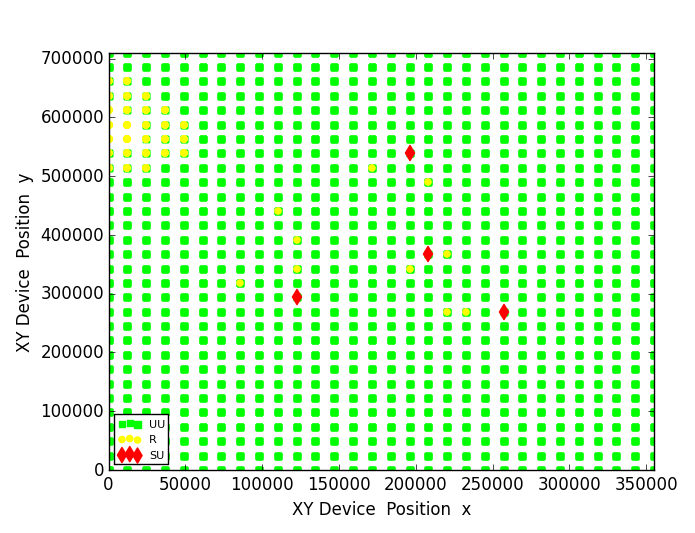
\includegraphics[width=.45\textwidth]{../plots/newplots/st-unroll-x-y-power-1.png}
          }
          ~
          \subfigure[Glitch source power between 30\% and 40\%]{
            \label{fig:st-unroll-x-y-offsets-2}
            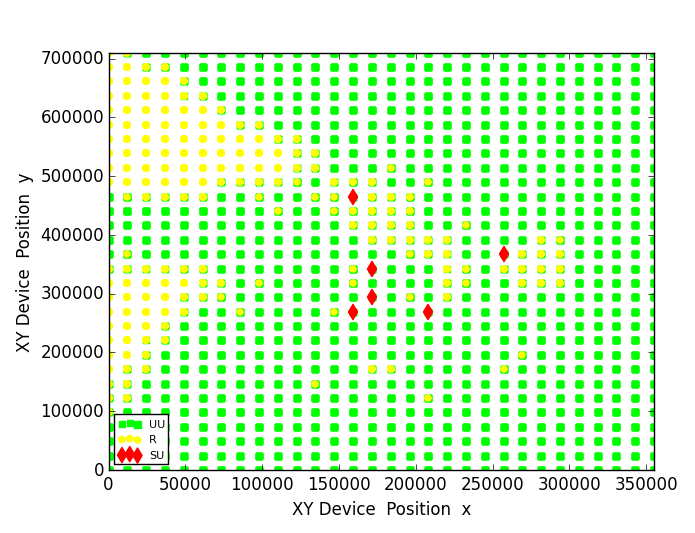
\includegraphics[width=.45\textwidth]{../plots/newplots/st-unroll-x-y-power-2.png}
          }
          \\
          \subfigure[Glitch source power between 50\% and 60\%]{
            \label{fig:st-unroll-x-y-offsets-3}
            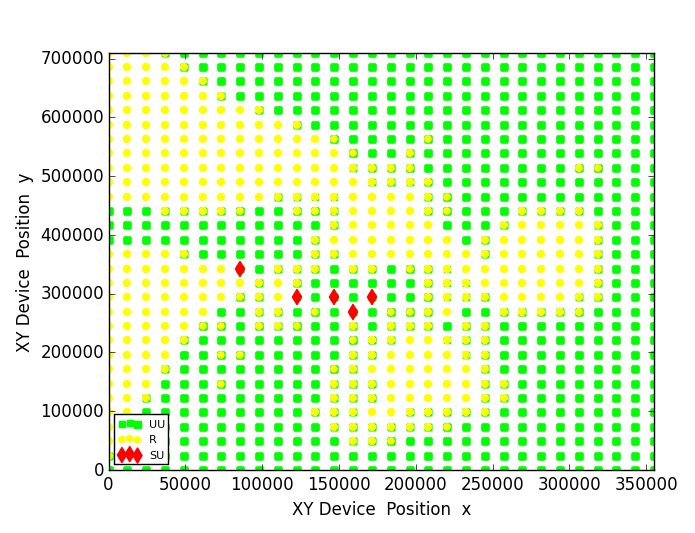
\includegraphics[width=.45\textwidth]{../plots/newplots/st-unroll-x-y-power-3.png}
          }
          ~
          \subfigure[Glitch source power between 70\% and 80\%]{
            \label{fig:st-unroll-x-y-offsets-4}
            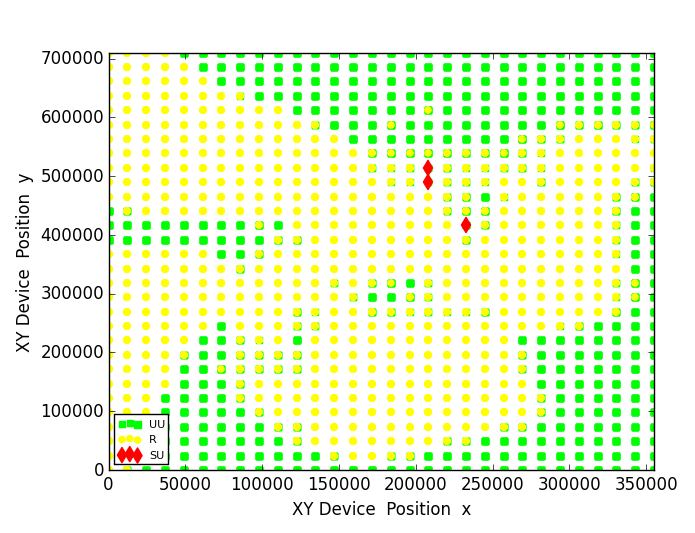
\includegraphics[width=.45\textwidth]{../plots/newplots/st-unroll-x-y-power-4.png}
          }
          \caption{X,Y plot, binned in two different ways, narrow parameters for \TI EM \unroll}
          \label{fig:st-unroll-x-y-offsets}
        \end{figure}

        \paragraph*{Glitch source power and position}
          By varying the position of a glitch, a point is hit by electromagnetic fields of different characteristics. This means that a glitch at different points with different powers can affect the same point. This is another explanation for the variance in location observed in the plots of \autoref{fig:st-unroll-x-y-offsets}.


    \subsubsection{Fixed parameters }

      Some parameters might affect the success rates of a glitch, but were not considered for this work, as this was not necessary to obtain successful results.  

        \paragraph*{Glitch repetition}
          Multiple faults can be injected during a single measurement by injecting multiple glitches. This was not required, as a single glitch can already achieve undetected successful faults. Some effort has been spent on performing dual fault experiments on the \TI with power glitching -- this showed that multiple faults are to the detriment of the success rate of the faults. This is interesting, as intuitively one might expect that multiple cores require multiple faults -- one for each core. Or perhaps one glitch to disturb the execution of the targeted instruction, and another fault to prevent the comparison from being successful. 

          As with all fault injection experiments, one can only theorize on the exact reason for this behavior. 
          As explained in \autoref{sec:background-countermeasures}, the cores execute the same instructions with a delay. Depending on the glitch that caused the fault, in an ideal situation a single fault will affect at most two instruction executions directly, two faults can affect at most four executions, three faults at most six executions, and so on. This increase in amount of instructions affected is a possible explanation for the increase in detection.
        \paragraph*{Z position}
          The Z position of the probe has not been altered throughout the experiments -- it remained in a fixed position as close as possible to the chip. Other research \cite{moro_electromagnetic_2013} notes that varying the Z position of the probe will have a similar effect to varying the glitch power. 
        \paragraph*{Coil size}
          By varying the size of the coil at the end of the EM probe, a more or less focused EM field can be achieved. For these experiments a 4 mm diameter coil is used, which provided successful faults and did not require tuning. 
        \paragraph*{Pulse polarity}
          The direction of the coil can change the polarity of the EM field. For these experiments a positive polarity coil was used and this did not require further tuning.

\newpage
\section{Breaking JTAG protection}
\label{sec:realistic-attack}

  As described in \autoref{sec:jtag-explanation}, steps in a fault injection attack targeting a debugging interface get fairly specific, more so than is the case with the characterization experiments discussed in \autoref{sec:characterization-results}, because every manufacturer implements the protection mechanisms in their own way. For the targets that are discussed here, their particular protection mechanisms can be found in \autoref{sec:targets}. In this section, in addition to the results of the fault injection attack, the steps leading up to finding these results are also discussed in more detail than they are discussed for the characterization experiments, as these steps are not as generic as the method for achieving the same in the characterization experiments. These steps mostly relate to identifying the moment in time where a fault should be injected and finding a reliable trigger signal to reach this point in time. 

  One successful attack that circumvents debugging interface protection has been performed for this work. In particular on the \TI, by using the power glitching technique. The \ST has not been evaluated in this way, due to time constraints. Some pointers on how a successful result can also be obtained on that target are given in this section.

  In parallel to this work, a similar type of attack was performed on a microcontroller targeting the same context as the \TI and the \ST, but only adhering to the simplest classification, QM. For reference, the results of this target can be found in \autoref{apdx:results}. The final success rate of bypassing the protection for this target is \textasciitilde80\%.

  \subsection{\TI}


  \subsubsection{Determining glitch trigger and glitch point}
    \label{sec:jtag-setup}
    In order to identify possible points where JTAG protection is happening, the power consumption during a boot sequence has been monitored with a Current Probe and an oscilloscope.  This shows a long period of \textasciitilde200ms where no activity is shown through the power consumption and a short 450\SI{}{\micro\second} window at the end of the boot sequence where activity is visible. This is likely where the more complicated initialization -- such as locking JTAG access -- occurs. The length of this window also roughly corresponds with the \textasciitilde3500 cycles reported by the datasheet \cite{texas_instruments_datasheet_2015} required for the power-up sequence. This window is shown in \autoref{fig:jtag2-trace1}.  

    \begin{figure}[H]
      \centering
      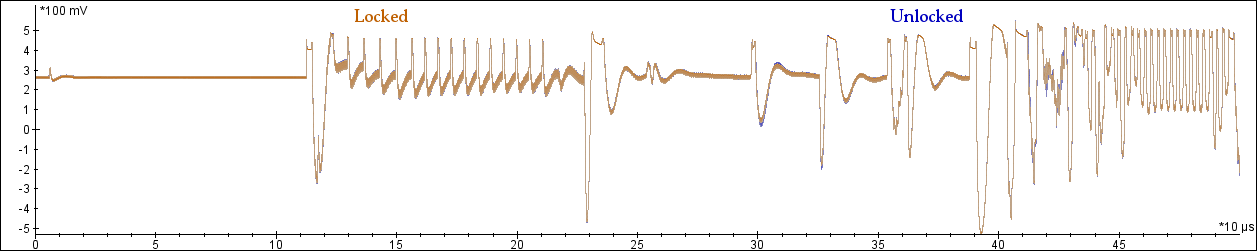
\includegraphics[width=\textwidth]{../plots/tms57-trace1.png}
      \caption{Interesting \SI{450}{\micro\second} window of power usage during power-up sequence}
      \label{fig:jtag2-trace1}
    \end{figure}

    As mentioned in \autoref{sec:target-ti}, an unlocked device exhibits different behavior than a locked device. This difference in behavior depending on the locked state might be visible in the power consumption at boot time, which is what is investigated to further narrow down this window -- 
    measuring the consumption of the boot process of both states 1,000,000 times and averaging the results per state. Overlaying both averaged results gives \autoref{fig:jtag2-trace1}. Through simple differential inspection, a small window of \textasciitilde\SI{10}{\micro\second} can be identified where significant difference in power consumption is present between a locked and an unlocked target, as shown in \autoref{fig:jtag2-trace2}. This is window is of a size where the simple random testing of parameters is feasible.


    \begin{figure}[H]
      \centering
      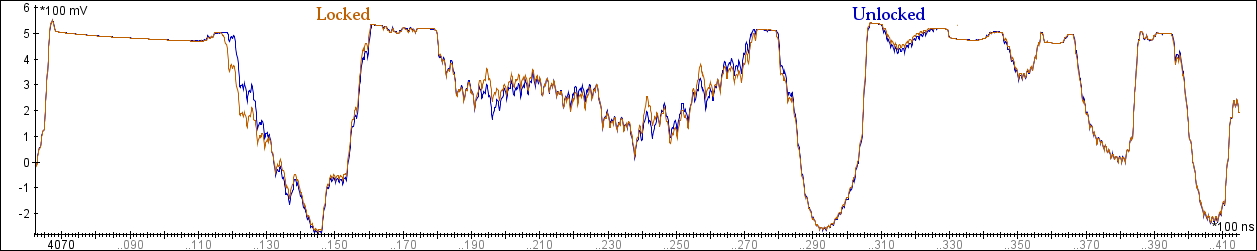
\includegraphics[width=\textwidth]{../plots/tms57-trace2.png}
      \caption{Difference between locked chip (brown) and unlocked chip (blue) in \SI{10}{\micro\second} window}
      \label{fig:jtag2-trace2}
    \end{figure}

    A trigger signal that has a reliable offset with the identified window is difficult to obtain. 
    A good option is passively monitoring EM emissions and triggering based on patterns observed in these emissions. The same can be done with power consumption, however obtaining power measurements that are as precise as in \autoref{fig:jtag2-trace1} is no longer an option: the measurements are obtained by monitoring the current with a coil, sending the power glitch through a coil will effectively filter it out. Power consumption could be observed by solely monitoring the voltage, but this produces a much lower quality signal.
    However, for the pattern recognition tool used in this attack this lower quality of the signal is not a problem, as the signal leaks enough information to reliably generate a trigger. This -- the approach of monitoring the voltage signal -- has been used in this attack, as it does not require any EM tools in addition to the power glitching tools.

    In order to test whether a fault was successful, the Uniflash debugging tool released by Texas Instruments is used. In this attack, the tool attempts to read a section of memory -- the part where the JTAG password value resides. Normally, this results an error, as the JTAG access is locked. Successful faults unlock the JTAG and allow for reading the value \texttt{effd ffff ffff ffff fffd fffe ffef fffe}, which is the password programmed to the target. Additionally, the signal on \errorpin is monitored to determine whether a fault was detected or not, using the patterns described in \autoref{fig:ti-error-traces}.


  \subsubsection{Results overview}

    After identifying the window of time during which a fault should be injected, finding a reliable trigger relative to this window and determining a way of classifying fault injection attempts, a strategy similar to the strategy applied in \autoref{sec:characterization-results} can be applied to tune all the glitch parameters. That is, start the attack with broad parameter settings and narrow these down based on the results obtained with the broad settings. The findings of these different configurations are given in \autoref{tab:ratesjtag2}. For the corresponding parameters, see \autoref{apdx:parameters}. 

    \begin{table}[H]
    \centering
    \begin{tabular}{lrrrr}
      \toprule
      Category    & Widest & Wider & Narrow & Single \\
      \midrule                                                                                                                                   
        \UU    
        & 51.13\% & 40.00\% & 52.48\% & 80.03\% \\
        \R   
        & 48.27\% & 54.36\% & 20.61\% & 14.06\% \\
        \UD  
        & 0.582\% & 5.437\% & 24.97\% & 3.289\% \\
        \SD     
        & 0.0007\% & 0.112\%  & 0.958\%  & 1.227\%  \\
        \SU      
        & 0.0003\% & 0.080\%  & 0.958\%  & 1.380\%  \\
      \bottomrule
    \end{tabular}
    \caption{\TI \jtag detection and success rates} 
    \label{tab:ratesjtag2}
    \end{table}

    While it is possible to find parameters for which a fault successfully bypasses the JTAG protection mechanism, it was not possible to find parameters for which detection is completely avoided at the same time during these experiments. In the best case found in this work, \textasciitilde4.5\% of the glitches cause a detected fault, while \textasciitilde1.4\% of the faults are both successful and undetected. This is significantly lower than the rate obtained for the simpler QM target of  \textasciitilde80\%. However, successful attacks attacks are still perfectly viable, even with this lower rate of success. Depending on how the detected faults are handled, an attacker might need multiple targets to successfully open the JTAG. 

  \subsubsection{Analysis of parameters}

    The effect of parameters individually and together is in line with the observations already described in \autoref{sec:characterization-observations}, as can be seen in \autoref{fig:ti-jtag-voltage-length} and \autoref{fig:ti-jtag-voltage-offset}. \autoref{fig:ti-jtag-voltage-length} reveals that the \TI exhibits the same type of relationship between glitch length and glitch voltage. Interestingly slightly `stronger' glitches are required to have an effect on the chip, compared to the glitches that caused and effect in \autoref{sec:characterization-observations}. The `shape' of the boundary area is also different -- instead of a single curved boundary, there seem to be two boundaries. As addressed in \autoref{sec:characterization-observations}, a definitive answer on why this is the case is hard to determine. 

    \begin{figure}[H]
      \centering
      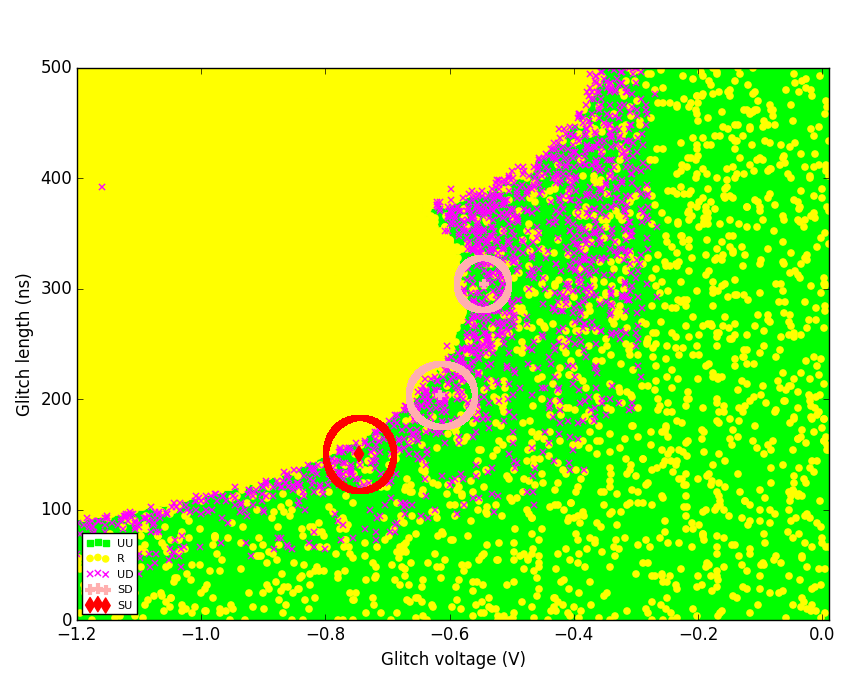
\includegraphics[width=\textwidth]{../plots/newplots/ti-jtag-voltage-length.png}
      \caption{\TI \jtag glitch voltage vs. length}
      \label{fig:ti-jtag-voltage-length}
    \end{figure}

    \autoref{fig:ti-jtag-voltage-offset} shows that there are distinct offsets at which a fault is detected, revealing that certain moments during the boot sequence are possibly sensitive to fault injection. The figure also shows that a very distinct moment in time exists where a successful fault can occur. 

    \begin{figure}[H]
      \centering
      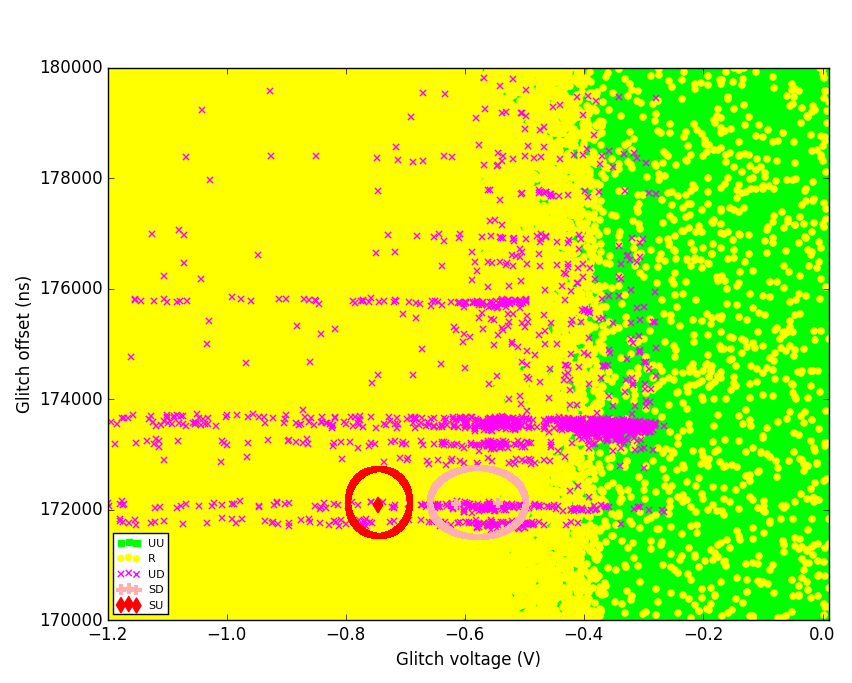
\includegraphics[width=\textwidth]{../plots/newplots/ti-jtag-voltage-offset.png}
      \caption{\TI \jtag glitch voltage vs. offset}
      \label{fig:ti-jtag-voltage-offset}
    \end{figure}

  \subsection{\ST}

    The \ST JTAG protection has not yet been evaluated -- this is considered future work. The available documentation reveals that the configuration scheme offers many points where fault injection can be an effective method to disrupt this stage. For example, configuration values are transferred from flash memory to their intended destinations -- this includes the password value. Injecting a fault at this moment can cause the process to be disrupted, leaving the target in a state where no password value reached the protection system.

\newpage
\section{Recommended mitigations and future work}
\label{sec:mitigations+futurwork}

  The results of the characterization experiments of \autoref{sec:characterization-results} show that safety mechanisms introduced in current ASIL-D certified microcontroller units are not adequately effective as countermeasures against fault injection attacks by themselves. They can, however, be a part of a defense strategy against fault injection attacks. 

  A proper defense strategy does not rely on a single countermeasure -- instead it takes a layered approach. Defense should start at the low level. Countermeasures at the most basic level start by protecting against glitches that occur naturally -- for example PLLs that ensure the clock stays in sync also mitigate clock signal based fault injection attacks, or capacitors whose purpose is to provide a stable power supply to the target also filter out weaker power glitches. Furthermore, low-level protection measures are found to specifically target fault injection attacks -- for example light sensors to mitigate attacks that involve optical techniques. 

  More intricate hardware countermeasures are the ones that are investigated in this work -- for example the lockstep configuration of two cores and the error correction and detection codes in memories. This research shows that even these countermeasures require additional work to adequately mitigate fault injection attacks.

  A solution that remains in the hardware domain is implementing higher levels of redundancy. In \citet{bar-el_sorcerers_2006} several other solutions besides the `Simple Time Redundancy with Comparison' are proposed. Examples of this are shifting or swapping the duplicated inputs before processing them, or adding more than one redundant processing unit (`Multiple  Time  Redundancy  with Comparison'). The latter offers opportunities for more elaborate schemes besides simply comparing outputs and notifying upon discrepancies: majority voting systems can be added to allow for fault recovery. 
  However, the effectiveness of hardware based countermeasures is up in the air. As covered in this work, the lockstep countermeasures is expected to have a very reasonable detection rate. The experimental work shows, however, that this rate is not so high. Therefore it is expected that similar hardware countermeasures with different parameters will also show similar effectiveness. Investigation of this is considered future work.

  Countermeasures can also be implemented in software. As mentioned in \autoref{sec:background-countermeasures}, several trade-offs have to be made when deciding on where to implement countermeasures, and to what extent. Primary trade-offs are increased production cost of for hardware countermeasures and increased latency in software countermeasures.
  Software countermeasures can be similar to the more intricate hardware measures mentioned before, like duplicate execution of a (set of) instructions and comparing their results. This can be tuned with multiple repeat executions and varying the inputs with shifts and masks. Other typical countermeasures include:
  \begin{itemize}
    \item introducing random delays in the entire execution of an application or in certain critical parts to complicate timing of a glitch; 
    \item double or triple checking values to require multiple faults for a successful result;
    \item utilizing the entire bit-space of a value, contrary to the usual approach where no bits set indicate logical false, while all other bit configuration indicate logical true, to require multiple bit-flips; 
    \item checking values to be within sensible ranges.
  \end{itemize}
  \noindent Note that, given enough information of an implementation, software countermeasures can typically be bypassed. They merely complicate -- possibly to acceptable levels -- matters for an attacker. Multiple checks can be bypassed by multiple faults, but finding the right parameters for multiple faults can render the attack infeasible due to the time required to find these parameters.

  Other pointers for future work are:

  \begin{itemize}
    \item Investigate the relationship between lockstep parameters, such as delay between cores \cite{tummeltshammer_analysis_2009}, amount of cores (\cite{ag_products} uses triple core lockstep), and detection rates. 
    \item Investigate the impact that software countermeasures have on the safety mechanisms such as lockstep en error control codes, by performing experiments with the hardware mechanisms turned on and turned off, while running the software countermeasures. 
  \end{itemize}

\newpage
\section{Conclusions}
\label{sec:conclusion}
  
  The purpose of this work is to address the question,

  \begin{quote}
    What is the current state of the security of the microcontrollers used in the automotive industry with respect to fault injection attacks?
  \end{quote}

  \noindent This question is divided it two subquestions. The first, 
    
  \begin{quote}
    What are the common automotive attacker scenarios that can utilize fault injection attacks?
  \end{quote}

  \noindent is addressed in \autoref{sec:attacker-scenarios}. The primary purpose of fault injection attacks is to bypass some sort of check related to security. As it turns out, such a building block can form an important piece in different kinds of scenarios related to the automotive context. Most prominently, such attacks enable attackers to extract firmware from microcontrollers. These firmwares can aid in further attacks, ranging from physical unauthorized attacks, to remotely exploitable vehicles en masse. Additionally, these firmwares are valuable assets themselves, as they are the result of years of work and research.

  To answer the second subquestion,

  \begin{quote}
    To what extent are advanced hardware attacks that use fault injection mitigated by safety mechanisms found in the automotive industry?
  \end{quote}

  \noindent two ASIL-D certified microcontroller units were selected as described in \autoref{sec:methodology}. ASIL is the risk classification introduced in the ISO26262 standard, grade D imposes the most stringent requirements. The manufacturers of these microcontroller units offer a development board that implements all its external capabilities, offering a fair platform for evaluating how their safety mechanisms hold up as countermeasures in a realistic fault injection attack setting.

  By applying two common techniques for fault injection -- power glitching and EM glitching -- the effectiveness of the safety mechanisms found in these targets were evaluated as countermeasures against fault injection. This has been done in two settings: one where a simple series of addition instructions is targeted and a second where a conditional branch is running. The first is to evaluate sensitivity to the glitching technique in a setting as simple as possible, while the second indicates the susceptibility to the technique in a more realistic piece of software. 


  The first target, the \TI, is highly susceptible to faults caused by power glitching, obtaining success rates as high as 60\% for the conditional branch experiment, as discussed in \autoref{sec:characterization-results}. For verification, EM glitching was also applied successfully, obtaining a success rate of 0.2\%. Narrowing down the parameters of this technique should yield similar results to the power glitching technique.

  The second target, the \ST, could not be successfully attacked with fault injection through power glitching. The power domain that powers the core can not be provided externally, as is the case with the \TI -- instead it is converted from the IO power input by means of a internal switching regulator. This filters out the power glitches injected by the attacker. Further investigation into a suitable injection point has to be performed. However, this regulator is no problem for the EM glitches, evidenced by the 58\% success rate obtainable for the conditional branch experiment.

  In addition to the characterization setting, the \TI has been the subject of another type of experiment, which is the topic of \autoref{sec:realistic-attack}. The \TI implements a scheme to protect access to its debugging interface (like most modern day microcontrollers). By applying fault injection at the right moment, this scheme can be bypassed. Access to a debugging interface potentially enables an attacker to read the firmware stored on the microcontroller and to write new firmware to it. Successful faults are slightly harder to obtain in this setting -- only 1.4\% of all the attempts under the best identified parameter configuration. Note that this percentage is still well within feasibility margins for an attacker. The \ST has not been evaluated in a similar fashion, only pointers to where such an attack might be successful are given in this work. \\

  \noindent In summary, this work shows that, while safety mechanisms can be a valuable part of a successful line of defense, by no means are they exhaustive and one should rely on other countermeasures as well to provide a proper defense against fault injection attacks. Which countermeasures and at what level must be the result of a carefully considered trade-off between several factors such as cost, latency and ease of patching. 


%% synced from zotero firefox
\newpage
\bibliography{../refs}

\newpage
\begin{appendices}

  \newgeometry{left=1cm,bottom=1cm,top=1cm,right=1cm}
  \pagenumbering{gobble}

  \section{Results table}
  \label{apdx:results}

  \begin{table}[H]
    \centering
    \begin{tabular}{ll rr rr rr rr}
    \toprule

      &  & \multicolumn{2}{c}{Widest }     &    
           \multicolumn{2}{c}{Wide }      &    
           \multicolumn{2}{c}{Narrow }   &
           \multicolumn{2}{c}{Single }  \\
           \cmidrule(lr){3-4}                    
           \cmidrule(lr){5-6}
           \cmidrule(lr){7-8}
           \cmidrule(l){9-10}
      Experiment & \multicolumn{1}{c}{Category}  & 
      \multicolumn{1}{c}{Counts}      & \multicolumn{1}{r}{\%}          & 
      \multicolumn{1}{c}{Counts}      & \multicolumn{1}{r}{\%}          & 
      \multicolumn{1}{c}{Counts}      & \multicolumn{1}{r}{\%}          & 
      \multicolumn{1}{c}{Counts}      & \%         \\

    \midrule

    \multicolumn{1}{c}{\multirow{3}{*}{ \parbox{2cm}{\TI power \unroll}}}

    & \UU    
    & 60048  & 38.26\%                   
    & &  
    & &     
    &  44  &  10.02\%   
    \\
    & \R   
    & 57436  & 36.60\%                   
    & &  
    & &     
    &  10  &  2.277\%   
    \\
    & \UD  
    & 15711  & 10.01\%                   
    & &  
    & &     
    &  0   &  0    \%   
    \\
    & \SD     
    & 22610  & 14.40\%                   
    & &  
    & &     
    &  0   &  0    \%   
    \\
    & \SU      
    & 1107   & 0.705\%                   
    & &  
    & &     
    &  384 &  87.47\%   
    \\

    \cmidrule(l){2-10}
    & total    
    & 156912 &                            
    & &  
    & & 
    &  438 &             
    \\       

    \midrule

    \multicolumn{1}{c}{\multirow{3}{*}{ \parbox{2cm}{\TI power \auth}}}
    & \UU    
    & 33669   & 19.83\%                     
    &  73543  & 43.82\%                 
    &  9445  & 82.35\%                 
    &  3186  & 34.27\%                      
    \\
    & \R   
    & 106323  & 62.62\%                     
    &  50751  & 30.24\%                 
    &  521   & 4.542\%                 
    &  493   & 5.303\%                      
    \\
    & \UD  
    & 26877   & 15.83\%                     
    &  32265  & 19.22\%                 
    &  1     & 0.008\%                 
    &  0     & 0    \%                      
    \\
    & \SD     
    & 2806    & 1.652\%                     
    &  10049  & 5.988\%                 
    &  2     & 0.017\%                 
    &  0     & 0    \%                      
    \\
    & \SU      
    & 94      & 0.055\%                     
    &  1200   & 0.715\%                 
    &  1500  & 13.07\%                 
    &  5616  & 60.41\%                      
    \\

    \cmidrule(l){2-10}
    & total    
    & 169769  &                           
    &  167808 &                       
    &  11469 &                       
    & 9295  &                                 
    \\

    \midrule

    \multicolumn{1}{c}{\multirow{3}{*}{ \parbox{2cm}{\TI EM \unroll}}}

    & \UU    
    & 8384   & 99.80\%                   
    &  188043 & 96.35\%    
    & & 
    & &
    \\
    & \R   
    & 13     & 0.154\%                   
    &  6492   & 3.326\%    
    & & 
    & &
    \\
    & \UD  
    & 2      & 0.023\%                   
    &  203    & 0.104\%    
    & & 
    & &
    \\
    & \SD     
    & 0      & 0    \%                   
    &  0      &  0    \%   
    & & 
    & &
    \\
    & \SU      
    & 1      & 0.011\%                   
    &  427    & 0.218\%    
    & & 
    & &
    \\

    \cmidrule(l){2-10}
    & total    
    & 8400   &                            
    &  195165 &             
    & & 
    & &
    \\   

    \midrule

    \multicolumn{1}{c}{\multirow{3}{*}{ \parbox{2cm}{\TI EM \auth}}}

    & \UU    
    & & 
    & & 
    & 38759  & 90.83\%  
    & &                            
    \\
    & \R   
    & & 
    & & 
    & 3801   & 8.907\%  
    & &                            
    \\
    & \UD  
    & & 
    & & 
    & 28     & 0.065\%  
    & &                            
    \\
    & \SD     
    & & 
    & & 
    & 0      & 0    \%  
    & &                            
     \\
    & \SU      
    & & 
    & & 
    & 82     & 0.192\%  
    & &                            
    \\

    \cmidrule(l){2-10}
    & total    
    & & 
    & & 
    & 8400   &           
    & &                            
      \\   
   
    \midrule

    \multicolumn{1}{c}{\multirow{3}{*}{ \parbox{2cm}{\ST EM \unroll}}}

    & \UU    
    & 23118  & 64.20\%
    & 88412  & 57.73\%  
    & & 
    & 2324 & 81.00\%                          
    \\
    & \R   
    & 12871  & 35.74\%
    & 64153  & 41.89\%  
    & & 
    & 0 & 0%                           
    \\
    & \SU      
    & 19     & 0.052\%
    & 572    & 0.373\%  
    & & 
    & 545 & 18.99\%                           
    \\

    \cmidrule(l){2-10}
    & total    
    &  36008  &           
    & 153137 & 
    &  & 
    & 2869&                           
      \\      

    \midrule

    \multicolumn{1}{c}{\multirow{3}{*}{ \parbox{2cm}{\ST EM \auth}}}

    & \UU    
    & & 
    & 97793  & 58.04\%        
    & 52433   & 28.68\%  
    & 4821 &   42.06\%        
    \\
    & \R   
    & & 
    & 70675  & 41.94\%        
    & 130125  & 71.19\%  
    & 0 &       0\%    
    \\
    & \SU      
    & & 
    &  9     & 0.005\%        
    &  213   & 0.114\%  
    & 6641   & 57.93\%           
    \\

    \cmidrule(l){2-10}
    & total    
    & & 
    & 168477  &                 
    & 182771  &          
    & 11462&           
    \\       


    \midrule

    \multicolumn{1}{c}{\multirow{3}{*}{ \parbox{2cm}{\NXP \jtag}}}

    & \UU    
    & 77295  & 87.05 \%               
    & 38536  & 85.05 \%            
    & 18185  & 21.97\%              
    & 2151   & 19.89\%               
    \\
    & \R   
    & 11404  & 12.84 \%               
    & 5804   & 12.81 \%            
    & 27874  & 33.68\%              
    & 0   & 0\%               
    \\
    & \SU      
    & 85     & 0.095 \%               
    & 965    & 2.130 \%            
    & 36678  & 44.33\%              
    & 8660   & 80.10\%               
    \\

    \cmidrule(l){2-10}
    & total    
    & 88784  &                        
    & 45305  &                     
    & 82737  &                        
    & 10811  &                        
    \\


    \midrule

    \multicolumn{1}{c}{\multirow{3}{*}{ \parbox{2cm}{\TI \jtag }}}
    & \UU    
    & 132562 & 51.13\%               
    & 18489   & 40.00\%            
    & 8321   & 52.48\%       
    & 28173  & 80.03\%             
    \\
    & \R   
    & 125152     & 48.27\%               
    & 25122   & 54.36\%            
    & 3268   & 20.61\%       
    & 4951   & 14.06\%             
    \\
    & \UD  
    & 1509       &  0.582\%                      
    & 2513    & 5.437\%            
    & 3960   & 24.97\%       
    & 1158   & 3.289\%             
    \\
    & \SD     
    & 2       &  0.0007\%                  
    & 52      & 0.112\%            
    & 152    & 0.958\%       
    & 432    & 1.227\%             
    \\
    & \SU      
    & 1      & 0.0003\%               
    & 37      & 0.080\%            
    & 152    & 0.958\%       
    & 486    & 1.380\%             
    \\

    \cmidrule(l){2-10}
    & total    
    & 259226 &                        
    & 46213 &                       
    & 15853 &                 
    & 35200 &                       
    \\
    \bottomrule
    \end{tabular}
    \caption{All results of each experiment}
    \label{tab:all-results}
  \end{table}

  \newpage

  \section{Parameter table}
  \label{apdx:parameters}

  \begin{table}[H]
    \centering
    \begin{tabular}{ll rr rr rr rr}
    \toprule

      &  & \multicolumn{2}{c}{Widest }     &    
           \multicolumn{2}{c}{Wide }      &    
           \multicolumn{2}{c}{Narrow }   &
           \multicolumn{2}{c}{Single }  \\
           \cmidrule(lr){3-4}                    
           \cmidrule(lr){5-6}
           \cmidrule(lr){7-8}
           \cmidrule(l){9-10}
      Experiment & \multicolumn{1}{c}{Parameter}  & 
      \multicolumn{1}{c}{Min}        & \multicolumn{1}{c}{Max}          & 
      \multicolumn{1}{c}{Min}        & \multicolumn{1}{c}{Max}          & 
      \multicolumn{1}{c}{Min}        & \multicolumn{1}{c}{Max}          & 
      \multicolumn{1}{c}{Min}        & \multicolumn{1}{c}{Max}          \\

    \midrule

    \multicolumn{1}{c}{\multirow{3}{*}{ \parbox{2cm}{\TI power \unroll}}}
      & Glitch length (ns)   
      & 0         & 300       
      &           &          
      &           &          
      & 260       & 260      
      \\
      \cmidrule(l){2-10}
      & Glitch offset (ns)   
      & 0         & 10000    
      &           &          
      &           &          
      & 1274      & 1274     
      \\ 
      \cmidrule(l){2-10}
      & Glitch voltage (V) 
      & -1        & -0.15    
      &           &          
      &           &          
      & -0.234    & -0.234   
      \\

    \midrule

    \multicolumn{1}{c}{\multirow{3}{*}{ \parbox{2cm}{\TI power \auth}}}
      & Glitch length (ns)   
      & 60      & 360      
      & 120     & 300      
      & 222     & 238      
      & 238     & 238        
      \\
      \cmidrule(l){2-10}
      & Glitch offset (ns)   
      & 30849   & 31165    
      & 30850   & 30940    
      & 30866   & 30902    
      & 30874   & 30874      
      \\ 
      \cmidrule(l){2-10}
      & Glitch voltage (V) 
      & -0.6      & -0.2   
      &-0.3       & -0.22  
      &-0.234     & -0.234 
      &-0.234     & -0.234   
     \\

    \midrule

    \multicolumn{1}{c}{\multirow{3}{*}{ \parbox{2cm}{\TI EM \unroll}}}
      & Glitch offset (ns)   
      & 0         & 1000   
      & 0         & 1000   
      &           &        
      &           &          
                \\
      \cmidrule(l){2-10}
      & Glitch power (\%)   
      & 0         & 30    
      & 10        & 50    
      &           &       
      &           &          
                \\
      \cmidrule(l){2-10}
      & X position   
      & 0         & 568582     % step 20
      & 170000    & 370000    % step 20
      &           &               
      &           &              
                \\
      \cmidrule(l){2-10}
      & Y position   
      & 0         & 519543    % step 20
      & 80000     & 330000   % step 25
      &           &              
      &           &             
                \\

    \midrule

    \multicolumn{1}{c}{\multirow{3}{*}{ \parbox{2cm}{\TI EM \auth}}}
      & Glitch offset (ns)   
      &           &        
      &           &        
      & 0         & 1000   
      &           &          
                \\
      \cmidrule(l){2-10}
      & Glitch power (\%)     
      &           &          
      &           &          
      & 10        & 50       
      &           &          
                \\
      \cmidrule(l){2-10}
      & X position   
      &           &          
      &           &          
      & 250000       & 370000  % step 20
      &           &          
                \\
      \cmidrule(l){2-10}
      & Y position   
      &           &          
      &           &          
      & 240000       & 320000 % step 25
      &           &          
                \\

    \midrule

    \multicolumn{1}{c}{\multirow{3}{*}{ \parbox{2cm}{\ST EM \unroll}}}
      & Glitch offset (ns)   
      & 10000     & 20000
      & 10000     & 15500 
      &           &        
      & 13414     & 13414    
      \\
      \cmidrule(l){2-10}
      & Glitch power (\%)     
      & 10        & 100       
      & 30        & 70        
      &           &           
      & 58        & 58      
      \\
      \cmidrule(l){2-10}
      & X position   
      & 0       & 355000   % step 30
      & 73400   & 220300   % step 39
      &         &          
      & 81131   & 81131    
      \\
      \cmidrule(l){2-10}
      & Y position   
      & 0       & 355000   % step 30
      & 122400  & 269300   % step 39
      &         &          
      & 207447  & 207447   
      \\

    \midrule

    \multicolumn{1}{c}{\multirow{3}{*}{ \parbox{2cm}{\ST EM \auth}}}
      & Glitch offset (ns)   
      &           &        
      &  100      &  5500   
      &  4850     &  4950
      &  4914     &  4914 
      \\
      \cmidrule(l){2-10}
      & Glitch power (\%)    
      &         &          
      & 20      &   80
      & 50      &   80 
      & 52      &   52 
      \\
      \cmidrule(l){2-10}
      & X position   
      &        &    
      & 73400   & 220300   % step 39
      & 122400  & 211306   %step 9
      & 133513  & 133513     
      \\
      \cmidrule(l){2-10}
      & Y position   
      &         &   
      & 122400  & 269300   % step 39
      & 146300  & 200300   % step 18
      & 176770  & 176770     
      \\


    \midrule

    \multicolumn{1}{c}{\multirow{3}{*}{ \parbox{2cm}{\NXP \jtag}}}
      & Glitch length (ns)   
      & 700     & 2000     
      & 700     & 2000     
      & 1250    & 1450     
      & 1330    & 1330     
      \\
      \cmidrule(l){2-10}
      & Glitch offset (ns)   
      & 17000   & 30000    
      & 19400   & 19900    
      & 19720   & 19820    
      & 19720   & 19820      
      \\
      \cmidrule(l){2-10}
      & Glitch voltage (V) 
%% synced from zotero firefox
      & -2.4    & -1.7     
      & -2.4    & -1.7     
      & -2.4    & -2.3     
      & -2.34   & -2.34      
      \\


    \midrule

    \multicolumn{1}{c}{\multirow{3}{*}{ \parbox{2cm}{\TI \jtag }}}
      & Glitch length (ns)   
      & 0       & 500      
      & 50      & 280      
      & 85      & 145      
      & 91      & 91         
      \\
      \cmidrule(l){2-10}
      & Glitch offset (ns)   
      & 170000  & 180000   
      & 172000  & 172200   
      & 172118  & 172124   
      & 172120  & 172120     
      \\
      \cmidrule(l){2-10}
  
      & Glitch voltage (V) 
      & -1.2    & -0.01    
      & -1.2    & -0.4     
      & -0.89   & -0.79    
      & -0.878  & -0.878     
      \\

    \bottomrule
    \end{tabular}
    \caption{All parameter settings for each experiment}
    \label{tab:all-params}
  \end{table}

  \newpage

  \section{\ST power glitching data}
  \label{apdx:st-power} 
    \begin{table}[H]
      \centering
      \begin{tabular}{ll rr}
      \toprule

        &  & \multicolumn{2}{c}{Widest }        
             \\
             \cmidrule(lr){3-4}                    
             
        Experiment & \multicolumn{1}{c}{Category}  & 
        \multicolumn{1}{c}{Counts}      & \multicolumn{1}{r}{\%}          
        \\

      \midrule

      \multicolumn{1}{c}{\multirow{3}{*}{ \parbox{2cm}{\ST through OSC / PMC input}}}

      & \UU    
      & 11463  & 10.00\%                   
      \\
      & \R   
      & 103113  & 89.99\%                   
      \\
      & \SU      
      & 0   & 0\%                   
      \\

      \cmidrule(l){2-4}
      & total    
      & 114576 &                            
      \\       

      \midrule

      \multicolumn{1}{c}{\multirow{3}{*}{ \parbox{2cm}{\ST through IO input}}}

      & \UU    
      & 82808  & 52.00\%                   
      \\
      & \R   
      & 76414  & 47.99\%                   
      \\
      & \SU      
      & 0   & 0\%                   
      \\

      \cmidrule(l){2-4}
      & total    
      & 159222 &                            
      \\       

      \bottomrule
      \end{tabular}
      \caption{\ST power glitching results}
      \label{tab:st-power-results}
    \end{table}

    \begin{table}[H]
      \centering
      \begin{tabular}{ll rr }
      \toprule

        &  & \multicolumn{2}{c}{Widest }     \\
             \cmidrule(lr){3-4}
        Experiment & \multicolumn{1}{c}{Parameter}  & 
        \multicolumn{1}{c}{Min}        & \multicolumn{1}{c}{Max}          \\

      \midrule

      \multicolumn{1}{c}{\multirow{3}{*}{ \parbox{2cm}{\ST through OSC / PMC input}}}
        & Glitch length (ns)   
        & 0         & 500       
        \\
        \cmidrule(l){2-4}
        & Glitch offset (ns)   
        & 4500      & 5200    
        \\ 
        \cmidrule(l){2-4}
        & Glitch voltage (V) 
        & -3.6      & -0.34    
        \\

      \midrule

      \multicolumn{1}{c}{\multirow{3}{*}{ \parbox{2cm}{\ST through IO input}}}
        & Glitch length (ns)   
        & 7         & 220       
        \\
        \cmidrule(l){2-4}
        & Glitch offset (ns)   
        & 2000      & 6000    
        \\ 
        \cmidrule(l){2-4}
        & Glitch voltage (V) 
        & -0.74      & -0.34    
        \\

      

      \bottomrule
      \end{tabular}
      \caption{\ST power glitching parameter settings}
      \label{tab:st-power-params}
    \end{table}


  \restoregeometry
\end{appendices}
\end{document}
